%----------------------------------------------------------------------------------------
% Preambulo y Configuración
%----------------------------------------------------------------------------------------

\documentclass[
    11pt,
    spanish,
    singlespacing,
    parskip,
    headsepline,
    bookmarks=true,
    unicode=true,
    pdftoolbar=true,
    pdfmenubar=true,
    pdffitwindow=false,
    colorlinks=true,
    linkcolor=blue,
    citecolor=blue,
    urlcolor=blue
]{MastersDoctoralThesis}

\usepackage[utf8]{inputenc} % Codificación de entrada UTF-8
\usepackage[T1]{fontenc}    % Codificación de salida para caracteres especiales
\usepackage{graphicx}       % Manejo de gráficos
\usepackage{eso-pic}        % Permite agregar fondos
\usepackage{hyperref}       % Manejo de hipervínculos y marcadores

% Redefinición de caracteres problemáticos en marcadores
\hypersetup{
    pdftitle={Título del Documento},
    pdfauthor={Autor del Documento},
    pdfkeywords={Sistemas Embebidos, Internet de las Cosas, Inteligencia Artificial},
    pdfstartview={FitH},
    unicode=true,
    colorlinks=true,
    linkcolor=blue,
    citecolor=blue,
    urlcolor=blue
}

\pdfstringdefDisableCommands{%
  \def\texttt#1{#1}%
  \def\textbf#1{#1}%
  \def\textit#1{#1}%
  \def\"{\"}%
  \def\~{~}%
  \def\'{'}%
  \def\^{}%
  \def\textunderscore{\_} % Manejo del subrayado en marcadores
}


% Último recurso de TeX para ajustar líneas rebeldes estirando los espacios,
% en lugar de desbordar el margen (solo actúa cuando no hay otra solución)
\setlength{\emergencystretch}{3em}

% Permitir que biblatex corte las URLs largas de la bibliografía
% (por defecto solo corta tras "//", lo que desborda el margen)
\setcounter{biburlnumpenalty}{9000}
\setcounter{biburlucpenalty}{9000}
\setcounter{biburllcpenalty}{9000}

% Estilo global de los bloques de código (listings)
\lstset{
    basicstyle=\small\ttfamily, % Un cuerpo menor que el texto: entran ~65 caracteres por línea
    breaklines=true,            % Corta las líneas largas en vez de desbordar el margen
    breakatwhitespace=true,     % Prefiere cortar en un espacio, no en mitad de una palabra
    breakindent=1em,            % Sangría de la continuación de una línea cortada
    keepspaces=true,            % Conserva la indentación original del código
    showstringspaces=false,     % No marca los espacios dentro de las cadenas
    captionpos=b,               % Epígrafe debajo del bloque
    aboveskip=1em,
    belowskip=1em
}

% Definir comandos requeridos por la clase
\newcommand{\degreename}{Maestría en Ciencias} % Cambia según tu título
\newcommand{\univname}{Universidad Nacional de Ejemplo} % Cambia según tu universidad
\newcommand{\keywordnames}{Palabras clave:}
%----------------------------------------------------------------------------------------
% Documento Principal
%----------------------------------------------------------------------------------------

\begin{document}

% Configuración de la portada
\posgrado{Carrera / Maestría}
\keywords{Sistemas Embebidos, Internet de las Cosas, Inteligencia Artificial}

% Incluir la portada desde un archivo separado
\include{portada}

% Configuración del contenido preliminar
\frontmatter % Usar numeración romana para las páginas preliminares
\pagestyle{plain} % Estilo de encabezado simple

%----------------------------------------------------------------------------------------
% Resumen
%----------------------------------------------------------------------------------------

\begin{abstract}
    \addchaptertocentry{\abstractname}
    El presente trabajo consiste en el diseño e implementación de un sistema que automatiza la recepción, interpretación y el procesamiento de los pedidos de un mercado de frutas y verduras recibidos a través de mensajería instantánea. El sistema captura pedidos en texto, voz o imagen, e identifica productos, cantidades y unidades mediante modelos de inteligencia artificial. Una vez estructurado el pedido, se imprime en el comercio mediante una impresora térmica conectada a un servidor local. El desarrollo fue realizado para la Tienda de frutas Luján, con el fin de reducir los tiempos operativos, disminuir los errores humanos y mejorar la trazabilidad de la gestión comercial.

    La solución se estructura sobre una arquitectura de cómputo distribuida entre el comercio y la nube, en la que las tareas críticas y de baja latencia se ejecutan localmente, mientras que las de mayor demanda de procesamiento se delegan a servicios remotos. El sistema se encuentra operativo en el comercio, donde procesa los pedidos en tiempo real y deja cada pedido listo para su preparación en menos de un minuto desde su recepción. Para su desarrollo se aplicaron conocimientos propios de la computación de borde, tales como la distribución del procesamiento entre el borde y la nube, la comunicación segura entre nodos, la actuación local sobre hardware y el diseño de soluciones de bajo costo.
\end{abstract}

%----------------------------------------------------------------------------------------
% Agradecimientos
%----------------------------------------------------------------------------------------

\begin{acknowledgements}
    \vspace{1.5cm}
    Quiero expresar mi agradecimiento a la Tienda de frutas Luján, y en particular a Marcos y Cristian Cestari, por la confianza depositada en este proyecto y por abrir las puertas de su comercio para el desarrollo y la validación del sistema. Su predisposición y su conocimiento del negocio fueron fundamentales para orientar el trabajo hacia una solución realmente útil.

    Agradezco también a mi director, Matías Martini, cuya orientación y experiencia en desarrollo de software e inteligencia artificial aplicada guiaron las decisiones técnicas a lo largo del desarrollo.

    Mi reconocimiento se extiende a mis compañeros y colegas, cuya colaboración fue esencial para superar los desafíos surgidos durante la implementación. Por último, agradezco a mis amigos y a mi familia, cuya paciencia y aliento incondicional fueron mi sostén durante este proceso, permitiéndome perseguir mis proyectos y crecer profesionalmente.
\end{acknowledgements}

%----------------------------------------------------------------------------------------
% Índice
%----------------------------------------------------------------------------------------

\tableofcontents
\listoffigures
\listoftables

%----------------------------------------------------------------------------------------
% Dedicatoria
%----------------------------------------------------------------------------------------

\dedicatory{A mi familia.}

%----------------------------------------------------------------------------------------
% Capítulos
%----------------------------------------------------------------------------------------

\mainmatter % Iniciar numeración numérica para el contenido principal
\pagestyle{thesis} % Estilo de encabezado de tesis

% Incluir capítulos desde archivos separados
% Chapter 1

\chapter{Introducción general} % Main chapter title

\label{Chapter1} % For referencing the chapter elsewhere, use \ref{Chapter1} 
\label{IntroGeneral}

En el presente capítulo se introduce el área en la que se enmarca el trabajo, se describe el contexto y la motivación que dieron origen al desarrollo, se revisan las soluciones existentes para problemas similares y se enuncian los objetivos perseguidos. El problema abordado es la gestión manual de los pedidos que los comercios reciben por canales de mensajería, y su resolución resulta relevante por el volumen de operaciones que hoy se procesan de esa forma.

%----------------------------------------------------------------------------------------

% Define some commands to keep the formatting separated from the content 
\newcommand{\keyword}[1]{\textbf{#1}}
\newcommand{\tabhead}[1]{\textbf{#1}}
\newcommand{\code}[1]{\texttt{#1}}
\newcommand{\file}[1]{\texttt{\bfseries#1}}
\newcommand{\option}[1]{\texttt{\itshape#1}}
\newcommand{\grados}{$^{\circ}$}

%----------------------------------------------------------------------------------------

%\section{Introducción}

%----------------------------------------------------------------------------------------



%----------------------------------------------------------------------------------------
%	SECTION 1
%----------------------------------------------------------------------------------------
 
\section{Mensajería instantánea y gestión de pedidos en comercios minoristas}
\label{sec:intro_general}
 
La creciente adopción de canales de mensajería instantánea como medio de contacto comercial modificó la forma en que los pequeños y medianos comercios reciben los pedidos de sus clientes. En el rubro de los mercados de frutas y verduras, gran parte de las ventas se gestiona a través de aplicaciones de mensajería, donde los pedidos llegan en formatos heterogéneos: texto libre, mensajes de voz, fotografías de listas manuscritas o capturas de pantalla. La interpretación de estos mensajes y su conversión en un pedido preparable constituyen, hoy, una tarea manual realizada por el personal del comercio.
 
El trabajo se sitúa en la intersección entre la automatización de procesos comerciales y la computación de borde (\textit{edge computing}), entendida esta última como el paradigma en el que parte del procesamiento y la toma de decisiones se ejecutan cerca del lugar donde se generan y se consumen los datos, en lugar de delegarse íntegramente a la nube. En un comercio minorista, el ``borde'' es el propio local: allí se recibe el pedido, allí debe imprimirse el ticket para su armado y allí ocurre la operación que no puede detenerse ante una caída de conectividad. Este enfoque contrasta con las arquitecturas puramente basadas en la nube, en las que todo el procesamiento se centraliza en servidores remotos.
 
El sistema desarrollado combina componentes de inteligencia artificial (IA) para la interpretación de los mensajes con una infraestructura de Internet de las cosas (IoT, del inglés \textit{Internet of Things}) para la actuación física en el local, articulados mediante una arquitectura híbrida que distribuye el cómputo entre un servidor local en el comercio y servicios alojados en la nube. El foco de esta memoria está puesto en los aspectos propios de la computación de borde: la distribución del procesamiento entre el borde y la nube, la comunicación segura entre ambos, la actuación local sobre hardware y las restricciones de costo, latencia y disponibilidad características de estos entornos. Los fundamentos de aprendizaje de máquina y aprendizaje profundo se asumen conocidos y no se desarrollan en detalle.
 
En la figura \ref{fig:diagrama_conceptual} se presenta un esquema conceptual de alto nivel del sistema, en el que el pedido ingresa por el canal de mensajería, se interpreta en la nube y deriva en la impresión local del ticket y en la visualización de la operación. La arquitectura detallada del sistema se describe en el capítulo \ref{Chapter3}.


 
\begin{figure}[htbp]
	\centering
	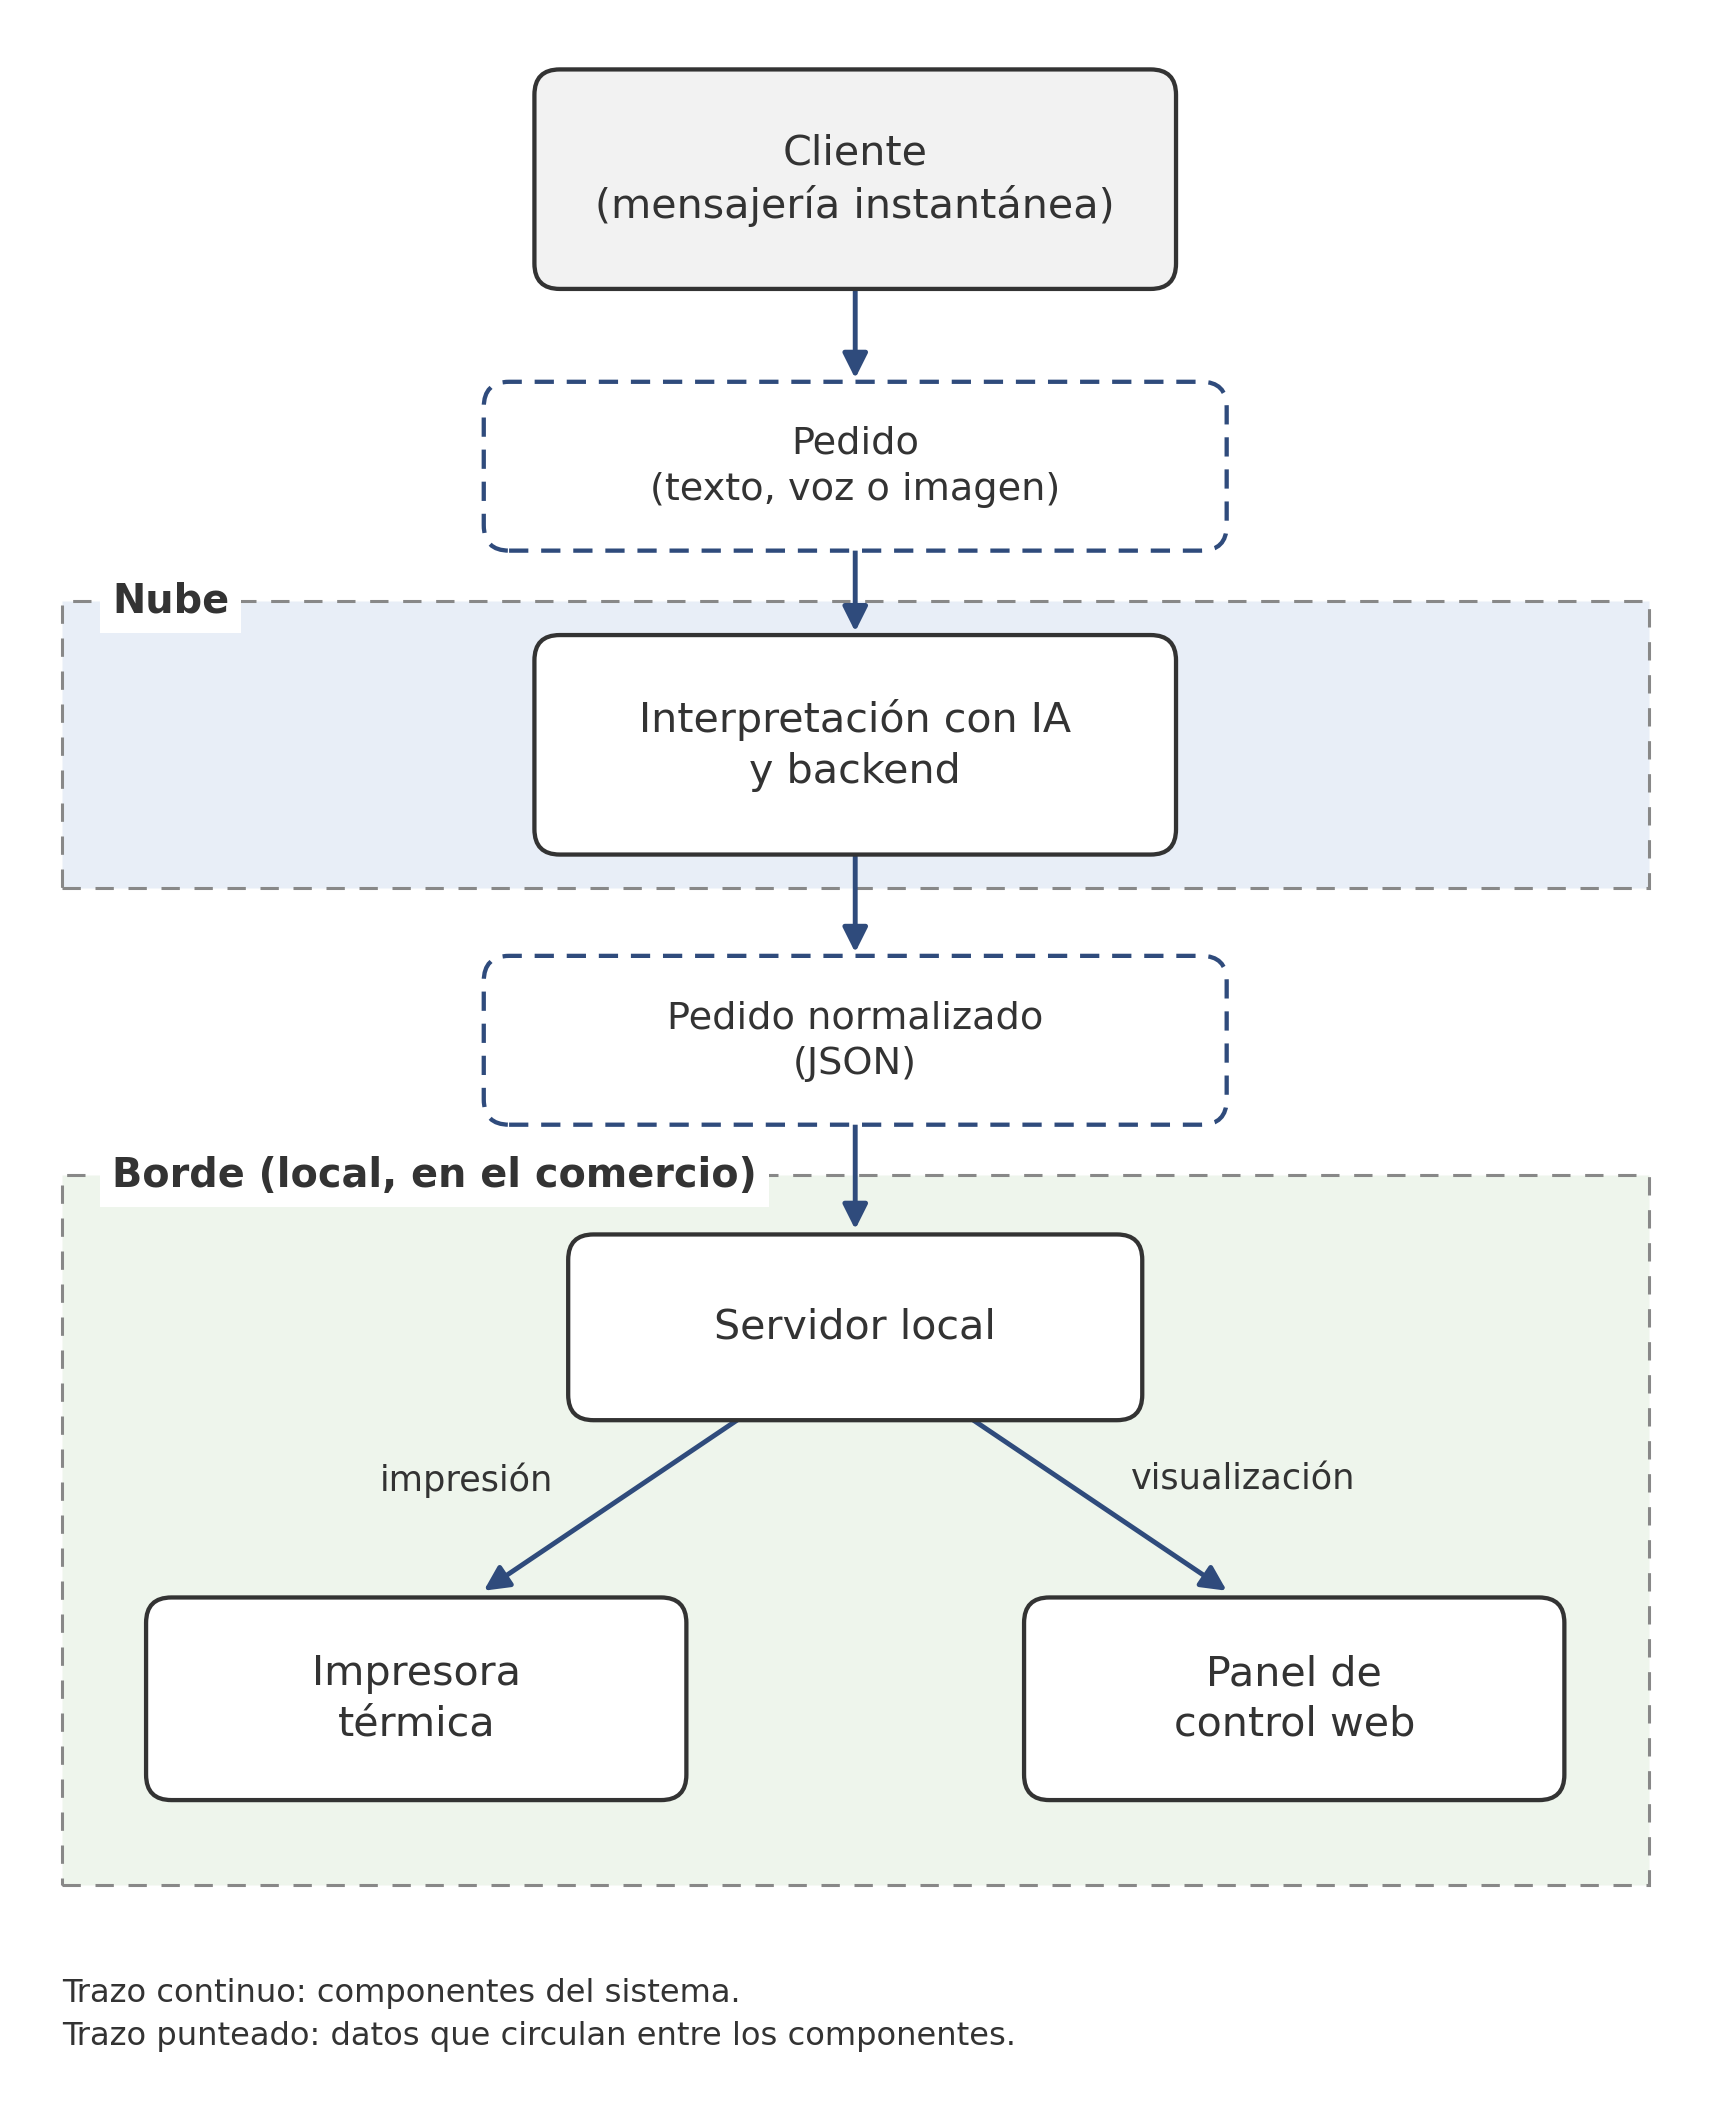
\includegraphics[width=0.9\textwidth]{Figures/diagrama_conceptual.png}
	\caption{Esquema conceptual del sistema: capas, componentes y flujo de datos.}
	\label{fig:diagrama_conceptual}
\end{figure}
 
%----------------------------------------------------------------------------------------
%	SECTION 2
%----------------------------------------------------------------------------------------
 
\section{Contexto y motivación}
\label{sec:contexto}
 
El trabajo se desarrolló para la Tienda de frutas Luján, un comercio minorista de frutas y verduras que recibe sus pedidos principalmente a través de mensajería instantánea. En la operación actual, un integrante del negocio lee cada mensaje entrante, interpreta su contenido (que puede llegar como texto, audio o imagen), normaliza los nombres y las cantidades de los productos y transcribe el pedido a un formato que permita su preparación y despacho.
 
Este proceso manual presenta varias limitaciones. En primer lugar, consume tiempo del personal que podría destinarse a la atención y a la preparación de los pedidos, y su capacidad se satura en los horarios de mayor demanda. En segundo lugar, la transcripción manual es propensa a errores de interpretación, especialmente ante mensajes de voz extensos, listas manuscritas poco legibles o denominaciones ambiguas de un mismo producto. En tercer lugar, al no existir un registro estructurado de los pedidos, se pierde trazabilidad: resulta difícil reconstruir el historial de un cliente, auditar un pedido puntual o extraer información agregada para la gestión comercial.
 
La motivación del desarrollo es, entonces, doble. Por un lado, se busca reducir los tiempos operativos y los errores humanos automatizando la recepción, la interpretación y la impresión de los pedidos. Por el otro, se procura hacerlo con una solución accesible y de bajo costo, adecuada a la realidad de un comercio que no dispone de infraestructura tecnológica avanzada ni de personal técnico especializado. Esta última condición es la que justifica el enfoque de computación de borde: procesar y actuar localmente permite que la operación crítica (la impresión del ticket para armar el pedido) siga funcionando con baja latencia y sin depender por completo de la disponibilidad de servicios remotos.
 
%----------------------------------------------------------------------------------------
%	SECTION 3
%----------------------------------------------------------------------------------------
 
\section{Estado del arte}
\label{sec:estado_arte}
 
La automatización de la recepción de pedidos en el comercio minorista puede abordarse desde distintos paradigmas, que se diferencian principalmente por dónde se ejecuta el procesamiento y por el grado de adaptación al canal de mensajería informal. A continuación, se revisan las alternativas existentes y se las contrasta con el enfoque adoptado en este trabajo.
 
\subsection{Soluciones basadas en la nube}
\label{subsec:soluciones_nube}
 
Una parte importante de las soluciones comerciales de gestión de pedidos y punto de venta se ofrece bajo el modelo de software como servicio, con todo el procesamiento centralizado en la nube. Entre las plataformas más conocidas se encuentran Shopify \cite{shopifypos} y, en el mercado local, Tiendanube \cite{tiendanubepdv}, que ofrecen soluciones de punto de venta y gestión de pedidos. Estas plataformas ofrecen paneles de administración, reportes y, en algunos casos, integración con canales de mensajería. Su principal ventaja es que no requieren infraestructura local más allá de un dispositivo con conexión a Internet. Sus limitaciones, en el contexto de este trabajo, son la dependencia total de la conectividad para operar, los costos recurrentes de suscripción y la escasa capacidad de personalización frente a un flujo de pedidos informal y no estructurado como el que se recibe por mensajería.
 
\subsection{Plataformas de automatización de mensajería}
\label{subsec:plataformas_mensajeria}
 
Existen plataformas y herramientas de automatización de flujos de trabajo que permiten conectar canales de mensajería con otros servicios mediante reglas o disparadores, como n8n \cite{n8n} o Zapier \cite{zapier}. Estas soluciones habilitan respuestas automáticas y la orquestación de tareas, pero por sí solas no resuelven la interpretación semántica de un pedido expresado en lenguaje natural, en audio o en una imagen. Para ello deben combinarse con modelos de procesamiento de lenguaje, reconocimiento de voz y reconocimiento óptico de caracteres (OCR, del inglés \textit{Optical Character Recognition}).
 
\subsection{Enfoques de borde e híbridos}
\label{subsec:enfoques_borde}
 
Frente a los esquemas puramente centralizados, la computación de borde propone ejecutar parte del procesamiento cerca del origen de los datos \cite{shi2016edge, satyanarayanan2017emergence}. En el comercio minorista, este enfoque resulta atractivo cuando existe una actuación física local, como la impresión de un ticket, que debe ocurrir con baja latencia y tolerancia a fallos de conectividad. Las arquitecturas híbridas, que combinan un nodo local con servicios en la nube, permiten equilibrar la capacidad de cómputo de la nube con la inmediatez y la resiliencia del procesamiento local \cite{tong2016hierarchical}.
 
\subsection{Comparación y posicionamiento del trabajo}
\label{subsec:comparacion_arte}
 
En la tabla \ref{tab:comparacion_arte} se comparan los tres paradigmas descriptos según los criterios más relevantes para el caso de uso abordado. El trabajo desarrollado se posiciona en el enfoque híbrido: delega en la nube las tareas de mayor demanda de cómputo (la interpretación de los mensajes mediante modelos de IA) y ejecuta en el borde la actuación crítica y de baja latencia (la impresión local del pedido), con lo que se busca un compromiso entre costo, personalización y disponibilidad adecuado a un comercio de baja complejidad tecnológica.
 
\begin{table}[h]
\centering
\caption{Comparación de paradigmas para la automatización de pedidos en el comercio minorista.}
\label{tab:comparacion_arte}
\begin{tabular}{p{3.2cm} p{2.6cm} p{2.6cm} p{2.6cm}}
\hline
Criterio & Nube pura & Automatización de mensajería & Enfoque híbrido (este trabajo) \\
\hline
Procesamiento local & No & Parcial & Sí (actuación local) \\
Dependencia de conectividad & Alta & Alta & Media \\
Personalización del flujo & Baja & Media & Alta \\
Costo de infraestructura & Bajo & Bajo & Bajo/Medio \\
Trazabilidad estructurada & Variable & Baja & Alta \\
\hline
\end{tabular}
\end{table}
 
%----------------------------------------------------------------------------------------
%	SECTION 4
%----------------------------------------------------------------------------------------
 
\section{Objetivos del trabajo}
\label{sec:objetivos}
 
El objetivo general del trabajo fue diseñar e implementar un sistema de automatización de pedidos. El sistema abarca la recepción, la interpretación y el procesamiento de los pedidos de un mercado de frutas y verduras recibidos a través de mensajería. De este modo se buscó reducir los tiempos operativos, minimizar los errores humanos y mejorar la trazabilidad de la operación comercial.
 
Para alcanzarlo, se definieron los siguientes objetivos específicos, formulados de manera concreta y verificable:
 
\begin{itemize}
	\item Capturar de forma automática los pedidos entrantes por el canal de mensajería, en sus distintos formatos: texto, voz e imagen.
	\item Interpretar el contenido de cada pedido mediante modelos de inteligencia artificial, identificando productos, cantidades y unidades, y normalizando denominaciones equivalentes de un mismo producto.
	\item Generar, a partir de esa interpretación, un pedido en formato estructurado y persistirlo de manera que quede registrada la trazabilidad completa, desde la recepción hasta la impresión.
	\item Imprimir automáticamente el pedido en una impresora térmica conectada a un servidor local, garantizando la actuación en el borde con baja latencia.
	\item Establecer una comunicación segura entre el servidor local y los servicios en la nube.
	\item Proveer un panel web que permita visualizar los pedidos en tiempo real, el historial y métricas básicas de operación.
	\item Validar el sistema en condiciones reales de operación en el comercio.
\end{itemize}
 
El alcance del trabajo se limita al flujo de recepción, interpretación, impresión y visualización de pedidos. Las tecnologías y componentes de terceros empleados en la construcción del sistema se describen en el capítulo \ref{Chapter2}, mientras que el diseño y la implementación de la arquitectura se detallan en el capítulo \ref{Chapter3}.
 
% !TEX root = ../memorianueva.tex
% Chapter 2

\chapter{Introducción específica} % Main chapter title

\label{Chapter2} % Para referenciar este capítulo: \ref{Chapter2}

En el presente capítulo se describen las tecnologías, plataformas, servicios y componentes de terceros utilizados como base para el desarrollo del sistema. Se presentan los dispositivos de borde, los protocolos de comunicación, las plataformas en la nube, los servicios de inteligencia artificial, las herramientas de almacenamiento y los recursos de visualización empleados en la solución.

%----------------------------------------------------------------------------------------
%	SECTION 1
%----------------------------------------------------------------------------------------

\section{Dispositivos de borde}
\label{sec:dispositivos_borde}

El nodo de borde del sistema está constituido por un servidor local instalado en el comercio y por una impresora térmica conectada a él. A diferencia de un sistema de Internet de las Cosas tradicional, no se emplean microcontroladores ni sensores. El dispositivo de borde es un equipo de cómputo de propósito general que ejecuta los servicios locales y comanda la impresión de los pedidos.

\subsection{Servidor local}
\label{subsec:servidor_local}

Como servidor local se utiliza una computadora con sistema operativo Windows Server 2019 \cite{windowsserver}, propiedad del cliente y preexistente en el local. Sobre este equipo se ejecutan el servidor de impresión y el cliente del túnel seguro hacia la nube.
% [PENDIENTE: si se conocen, agregar las características básicas del equipo
% (procesador, memoria).]

Se evaluaron dos alternativas para el nodo de borde. La primera consistió en incorporar una computadora de placa única (SBC, del inglés \textit{Single Board Computer}) dedicada, como una Raspberry Pi \cite{raspberrypi}. La segunda consistió en reutilizar el equipo ya disponible en el comercio. Se optó por la segunda opción por tres motivos. El primero fue el costo, dado que reutilizar el hardware disponible elimina la inversión marginal en equipamiento. El segundo fue la operación, ya que el equipo permanece encendido durante el horario comercial y resulta conocido por el personal, lo que simplifica la instalación y el mantenimiento. El tercero fue la compatibilidad, porque la impresora provee controladores para Windows y su integración no requirió desarrollos de bajo nivel.

Como contrapartida, un equipo de propósito general consume más energía que una SBC dedicada y puede verse condicionado por otros usos dentro del comercio. Esta limitación se consideró aceptable frente a la simplicidad operativa obtenida.

También se descartó el uso de un microcontrolador, ya que el conjunto de responsabilidades del nodo de borde (un servidor web local, el cliente del túnel seguro y la administración de la cola de impresión) se resuelve de manera más conveniente sobre un sistema operativo completo.

\subsection{Impresora térmica}
\label{subsec:impresora}

Para la impresión de los tickets se utiliza una impresora térmica Hasar P-HAS-181 \cite{hasar181}, un modelo de tipo comandera del fabricante argentino Grupo Hasar, orientado al punto de venta. La impresora imprime por cabezal térmico directo sobre rollos de papel de 80 mm de ancho y dispone de tres interfaces de conexión (puerto serie, USB y Ethernet) y de controladores para Windows. Sus comandos de impresión resultan compatibles con ESC/POS \cite{escpos}, el conjunto de instrucciones definido por Epson que constituye el estándar de facto del sector.

En la instalación actual, la impresora se conecta al servidor local por USB. La disponibilidad de una interfaz Ethernet fue, sin embargo, un criterio de selección. El equipo puede requerir un cambio de ubicación dentro del comercio, por ejemplo hacia el sector de armado de pedidos. La conexión por red permitiría ese traslado sin dependencia de la proximidad física con el servidor.

La elección de este modelo se fundamentó en cuatro factores. La impresión térmica es el estándar del comercio minorista por su velocidad y su bajo costo operativo, al no utilizar tinta ni cartuchos. La compatibilidad con ESC/POS permite comandar el equipo desde bibliotecas ampliamente disponibles, sin depender de un protocolo propietario. Los controladores para Windows garantizan la integración directa con el servidor local. Por último, se trata de un fabricante nacional, lo que asegura la provisión local de insumos, repuestos y servicio técnico, un criterio relevante para un comercio sin personal técnico propio.

%----------------------------------------------------------------------------------------
%	SECTION 2
%----------------------------------------------------------------------------------------

\section{Protocolos de comunicación}
\label{sec:protocolos}

El intercambio de mensajes entre los componentes se realiza mediante HTTP \cite{rfc9110}, con interfaces que siguen el estilo arquitectónico REST \cite{fielding2000rest}. La elección responde a que todos los servicios involucrados exponen sus funcionalidades a través de interfaces de programación de aplicaciones (API, del inglés \textit{Application Programming Interface}) basadas en HTTP. Para los eventos asincrónicos, como la llegada de un mensaje, se emplean notificaciones automáticas (\textit{webhooks}), que evitan que el sistema receptor deba consultar de forma periódica por novedades.

\subsection{Canal de mensajería}
\label{subsec:whatsapp}

La vinculación con WhatsApp se realiza mediante Evolution API \cite{evolutionapi}, una pasarela de mensajería de código abierto que expone las funciones de la plataforma a través de una interfaz REST y de notificaciones automáticas. Evolution API admite dos modos de conexión. El primero se basa en el protocolo de WhatsApp Web, mediante la biblioteca Baileys \cite{baileys}, y no requiere verificación comercial ante Meta. El segundo se basa en la API oficial WhatsApp Business Cloud \cite{whatsappbusiness}. En este trabajo se utiliza el primer modo. Ante cada mensaje entrante, de texto, voz o imagen, la pasarela emite una notificación con el contenido o con las referencias para descargarlo.

La elección de Evolution API para la etapa inicial del trabajo se fundamentó en su costo nulo, en su rapidez de puesta en marcha (no requiere verificación comercial ni aprobación de plantillas) y en su despliegue autoalojado, coherente con la infraestructura del sistema. Su principal limitación es que el modo basado en WhatsApp Web constituye un mecanismo no oficial, con posibles restricciones de estabilidad y cumplimiento. Por ese motivo, el sistema se diseñó compatible con la API oficial de WhatsApp Business, y la migración prevista no implica modificaciones estructurales en los flujos de procesamiento.

\subsection{Comunicación segura con la nube}
\label{subsec:cloudflare}

Para vincular los servicios en la nube con el servidor local sin apertura de puertos en la red del comercio, se emplea un túnel seguro provisto por Cloudflare \cite{cloudflaretunnel}. Un cliente ligero, ejecutado en el servidor local, establece una conexión cifrada saliente hacia la infraestructura del proveedor. A través de esa conexión, los servicios remotos alcanzan al nodo de borde.

Se consideraron dos alternativas. La apertura de puertos en el enrutador del local exige configurar el equipamiento de red y deja un servicio a la escucha de conexiones entrantes desde Internet, lo que amplía la superficie de ataque. Una red privada virtual (VPN, del inglés \textit{Virtual Private Network}) resuelve la seguridad, pero agrega administración de claves y configuración en ambos extremos. El túnel de Cloudflare, en cambio, no requiere configuración del enrutador, ya que la conexión es saliente, cifra el tráfico de extremo a extremo y mantiene la red interna sin exposición entrante, con una operación mínima acorde a un local sin personal técnico.

%----------------------------------------------------------------------------------------
%	SECTION 3
%----------------------------------------------------------------------------------------

\section{Plataformas cloud y servicios}
\label{sec:plataformas_cloud}

En esta sección se describen los servicios en la nube sobre los que se apoya el sistema, que comprenden la plataforma de orquestación de los flujos de procesamiento, la infraestructura donde se despliegan los componentes y los servicios de inteligencia artificial que resuelven la interpretación de los pedidos.

\subsection{Orquestación de flujos de trabajo}
\label{subsec:n8n}

La orquestación de las tareas de recepción, interpretación y estructuración de los pedidos se realiza con n8n \cite{n8n}, una plataforma de automatización de flujos de trabajo de código abierto. En n8n, la lógica se construye mediante la conexión de nodos configurables (disparadores, transformaciones e integraciones con servicios externos) en flujos visuales. Este enfoque permite integrar servicios heterogéneos sin desarrollar desde cero la lógica de integración. La plataforma incorpora además agentes de inteligencia artificial (\textit{AI Agents}), que encadenan modelos de lenguaje con herramientas y fuentes de datos. Sobre esa capacidad se apoya la interpretación de los pedidos.

Frente a alternativas comerciales de automatización en la nube, como Zapier \cite{zapier}, n8n presentó dos ventajas decisivas para este trabajo. La primera es la posibilidad de autoalojamiento en la propia infraestructura, sin costo por tarea ejecutada, un factor crítico dado el volumen diario de mensajes. La segunda es que los datos de los clientes permanecen dentro del entorno controlado por el sistema, sin atravesar una plataforma de terceros adicional.

\subsection{Infraestructura de despliegue}
\label{subsec:vps_docker}

Los servicios en la nube se alojan en un servidor privado virtual (VPS, del inglés \textit{Virtual Private Server}) del proveedor Hostinger \cite{hostinger}, en su plan KVM 4. Este plan provee 4 núcleos virtuales, 16 GB de memoria RAM, 200 GB de almacenamiento NVMe y 16 TB de transferencia mensual. El dimensionamiento respondió a la carga concurrente del sistema, ya que sobre el mismo servidor conviven la pasarela de mensajería, el motor de flujos, las bases de datos y el panel web.

Todos los servicios se despliegan de forma contenerizada mediante Docker \cite{docker}. La contenerización empaqueta cada servicio junto con sus dependencias en unidades aisladas y reproducibles, lo que permite describir el despliegue en archivos versionables, reproducir el entorno sin diferencias de configuración y actualizar cada componente de manera independiente.

\subsection{Servicios de inteligencia artificial}
\label{subsec:servicios_ia}

La interpretación de los pedidos requiere resolver tres tareas diferenciadas: convertir los mensajes de voz en texto, leer las listas manuscritas enviadas como fotografía y extraer de un texto informal los productos, las cantidades y las unidades solicitadas. Cada tarea se resuelve con un modelo de inteligencia artificial consumido como servicio en la nube, provisto por OpenAI \cite{openai} o por Anthropic \cite{claude}.

La transcripción de audio se realiza con el servicio de transcripción de OpenAI, basado en el modelo Whisper \cite{whisper}. Su característica más relevante para este trabajo es la robustez frente a condiciones adversas de grabación, como el ruido de fondo, la variabilidad de acentos y la calidad desigual del micrófono. Los mensajes de voz de los clientes se graban dentro del comercio o en la vía pública, sin control sobre el entorno sonoro, por lo que esa robustez resultó determinante.

La lectura de las imágenes se resuelve con modelos multimodales de visión. Se evaluó como alternativa un motor de reconocimiento óptico de caracteres (OCR, del inglés \textit{Optical Character Recognition}) clásico, pero las imágenes recibidas (listas manuscritas con caligrafías dispares e iluminación irregular, y capturas de planillas) le hacen perder precisión, porque opera sobre cada carácter de manera aislada y sin considerar la disposición del contenido. Los modelos multimodales, en cambio, interpretan la imagen en su contexto, reconocen la estructura tabular y aprovechan el conocimiento del dominio para resolver ambigüedades.

Sobre cada imagen se ejecutan dos modelos de proveedores distintos, GPT-4o de OpenAI y Claude Sonnet de Anthropic, porque ante una misma imagen producen en ocasiones lecturas discrepantes, sobre todo con caligrafías difíciles o planillas complejas. Las dos lecturas se reconcilian en un tercer paso, donde el modelo GPT-5.5 de OpenAI las compara, corrige las diferencias y devuelve una transcripción única. Esta redundancia agrega costo y latencia, pero reduce el riesgo de un error silencioso en la etapa más frágil de la interpretación.

La estructuración final se resuelve con un modelo extenso de lenguaje (LLM, del inglés \textit{Large Language Model}), GPT-5.5 de OpenAI, integrado como agente dentro del flujo. Recibe el texto del pedido junto con el catálogo del comercio y produce una representación estructurada con los productos, las cantidades y las unidades. Su capacidad de interpretar lenguaje informal, con abreviaturas, errores de tipeo y denominaciones no normalizadas, constituye el aporte central de estos modelos a la solución.

La decisión de consumir estos modelos como servicio, en lugar de ejecutarlos sobre la propia infraestructura, define la distribución del cómputo entre el borde y la nube. Los tres modelos exigen recursos de procesamiento muy superiores a los del nodo de borde, por lo que su ejecución local no resultaba viable con el equipamiento del comercio. Su consumo como servicio mantiene la inversión inicial y la complejidad operativa en el mínimo. El costo es doble: un componente variable por uso y la dependencia de la conectividad para la etapa de interpretación. La actuación crítica del sistema permanece en el borde, de manera que esa dependencia no compromete la operación local de impresión.

%----------------------------------------------------------------------------------------
%	SECTION 4
%----------------------------------------------------------------------------------------

\section{Herramientas de almacenamiento y visualización}
\label{sec:almacenamiento_visualizacion}

En esta sección se presentan las herramientas de persistencia de datos y los componentes destinados a la visualización de la operación. Las bases de datos que sostienen la información del sistema y el servidor local junto con el panel web de control.

\subsection{Bases de datos}
\label{subsec:bases_datos}

La información de pedidos, clientes y productos se almacena en PostgreSQL \cite{postgresql}, una base de datos relacional de código abierto. Su modelo relacional con integridad referencial resulta adecuado para el dominio del problema, donde los pedidos se vinculan con clientes y con artículos del catálogo. La trazabilidad exigida al sistema requiere garantías de consistencia transaccional, y las consultas sobre el historial alimentan además las métricas del panel de control.

De manera complementaria se emplea Redis \cite{redis}, una base de datos en memoria de tipo clave-valor, para la gestión de las sesiones y del estado de los clientes activos durante la recepción de un pedido. Redis ofrece tiempos de acceso muy bajos y expiración automática de claves, características apropiadas para datos de carácter transitorio con alta frecuencia de lectura y escritura. La combinación responde a un criterio de diseño explícito: los datos persistentes y auditables residen solo en la base relacional, mientras que Redis se reserva para información temporal, de modo que una eventual falla de la capa en memoria no compromete los registros del negocio.

\subsection{Servidor local y panel de visualización}
\label{subsec:flask_panel}

El servidor de impresión que se ejecuta en el nodo de borde se implementó sobre Flask \cite{flask}, un entorno de desarrollo web minimalista escrito en el lenguaje Python. Flask permite exponer servicios HTTP con una huella de recursos reducida y sin la complejidad de un servidor de aplicaciones completo. Resulta adecuado para un servicio local de propósito específico, que recibe el pedido estructurado y comanda la impresora sobre el equipo Windows del comercio.

La visualización de los pedidos, del historial y de las métricas de operación se ofrece a través de un panel web alojado en el VPS, accesible desde cualquier navegador moderno. Este enfoque evita la instalación de aplicaciones adicionales en los dispositivos del comercio. El panel se desarrolló con Angular \cite{angular}, un entorno de desarrollo de aplicaciones web mantenido por Google, junto con la biblioteca de componentes Angular Material. La representación de las métricas se resuelve con Chart.js \cite{chartjs}. La elección de un entorno estructurado, con tipado estático y organización por componentes, respondió a la necesidad de sostener el crecimiento del panel a medida que se incorporan nuevas vistas y funciones de administración.
% Chapter 3

\chapter{Diseño e implementación} % Main chapter title

\label{Chapter3} % Para referenciar este capítulo: \ref{Chapter3}

En el presente capítulo se describen el diseño y la implementación del sistema. Se presenta la arquitectura general y la distribución del cómputo entre el comercio y la nube. Luego se detalla cada capa: la captura de los pedidos, la conectividad entre los componentes, el procesamiento y la persistencia, la interfaz de usuario y las medidas de seguridad. En cada sección se exponen los problemas encontrados, los criterios adoptados y la justificación de las decisiones tomadas.

%----------------------------------------------------------------------------------------
%	SECTION 1
%----------------------------------------------------------------------------------------

\section{Arquitectura del sistema}
\label{sec:arquitectura}

El sistema se organizó en tres capas funcionales. La capa de captura y comunicación recibe los mensajes del canal de mensajería y los prepara para su interpretación. La capa de procesamiento inteligente interpreta el contenido, lo estructura contra el catálogo del comercio y lo persiste. La capa de interacción local e impresión ejecuta la actuación física sobre la impresora del negocio. En la figura \ref{fig:arquitectura_sistema} se presentan las tres capas, sus componentes y el flujo de datos extremo a extremo.

\begin{figure}[htbp]
  \centering
  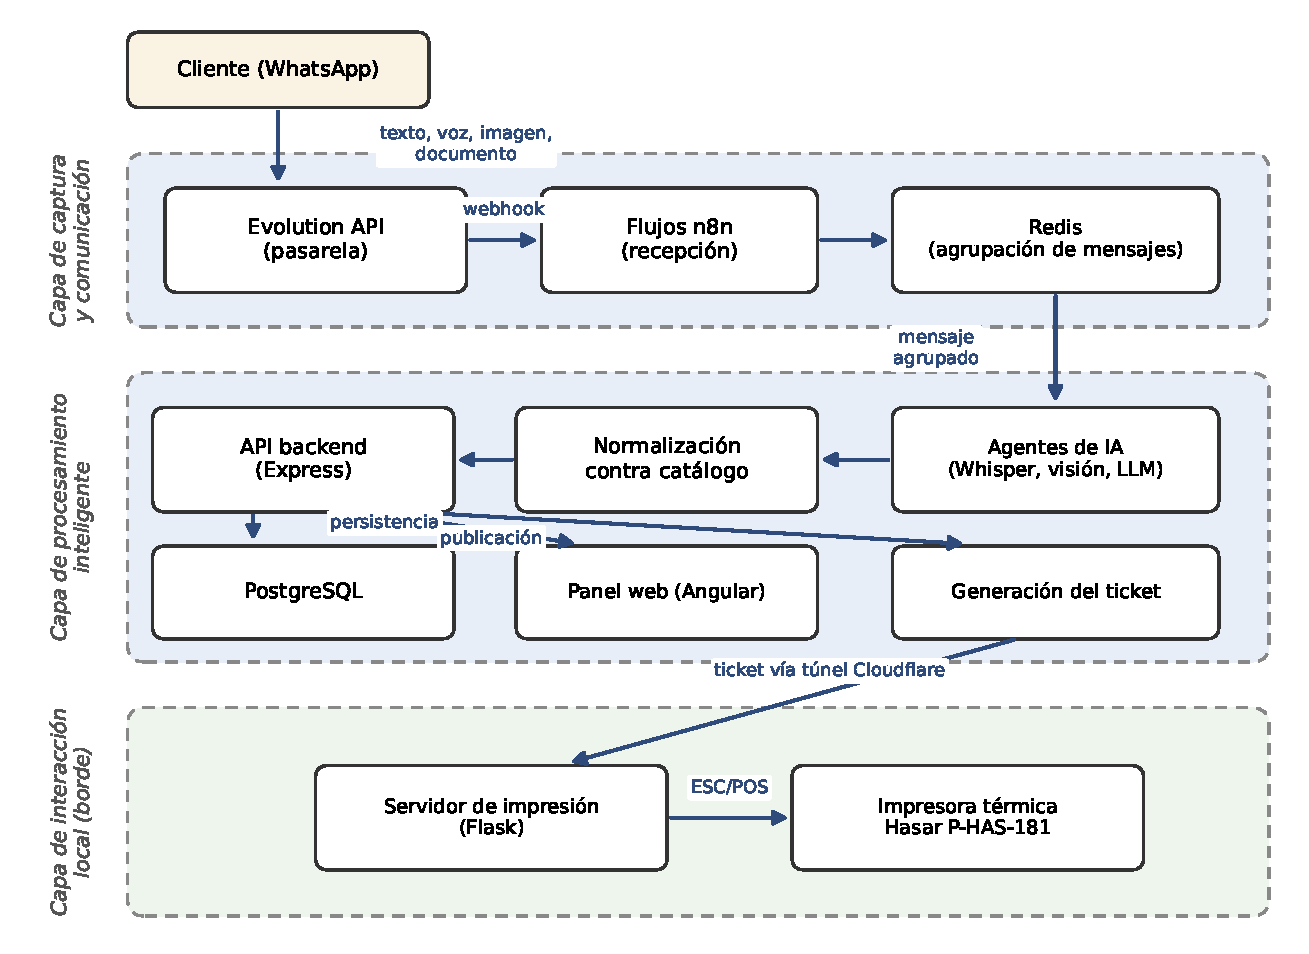
\includegraphics[width=\textwidth]{Figures/arquitectura_sistema.pdf}
  \caption{Arquitectura del sistema en tres capas.}
  \label{fig:arquitectura_sistema}
\end{figure}

\subsection{Criterio de distribución del cómputo}
\label{subsec:criterio_distribucion}

El criterio rector del diseño fue asignar cada tarea al lugar de ejecución que mejor equilibra latencia, disponibilidad y costo. Las tareas de mayor demanda de procesamiento son la transcripción de voz, la lectura de imágenes y la estructuración mediante modelos de lenguaje. Todas ellas se delegaron a servicios en la nube, donde la capacidad de cómputo resulta elástica y los modelos se consumen bajo demanda. Ejecutarlas sobre el equipo del comercio habría exigido una inversión en hardware incompatible con las restricciones económicas del proyecto.

La actuación crítica del negocio es la impresión del ticket que habilita el armado del pedido. Esa tarea se resolvió en el borde, sobre el servidor local del comercio. La decisión responde a tres motivos. El primero es la latencia: la orden de impresión recorre un único salto desde el servidor local hasta la impresora. El segundo es la independencia del canal: la impresora nunca se expone a Internet, sino que queda detrás de un servicio local que actúa como intermediario. El tercero es la continuidad operativa: el personal puede reimprimir un pedido ya recibido desde el panel sin que intervengan los modelos de inteligencia artificial.

\subsection{Organización del código}
\label{subsec:organizacion_codigo}

El código fuente se organizó en cuatro módulos independientes, que se corresponden con los componentes de la arquitectura:

\begin{itemize}
  \item \code{api/}: la interfaz de programación de aplicaciones (API) y la lógica de pedidos, implementadas con Node.js, Express y TypeScript sobre el mapeador objeto-relacional (ORM, del inglés \textit{Object-Relational Mapping}) Prisma.
  \item \code{web/panel/}: el panel web de control, desarrollado con Angular.
  \item \code{n8n/}: los flujos de automatización que orquestan la recepción y la interpretación de los pedidos.
  \item \code{print\_server/}: el servidor de impresión que se ejecuta en el nodo de borde, implementado con Flask.
\end{itemize}

Esta separación permite desplegar, actualizar y probar cada módulo por separado. La API y el panel se comunican solo a través de recursos HTTP, sin dependencias de código compartido, de modo que un cambio en la interfaz no obliga a modificar el servidor.

\subsection{Entorno de desarrollo}
\label{subsec:entorno_desarrollo}

El desarrollo planteó una dificultad práctica: la impresora se encuentra en el comercio y permanece en uso durante el horario comercial, por lo que no resultaba viable ensayar contra el equipo real cada modificación del flujo.

La solución adoptada fue una versión simulada del servidor de impresión. Ese componente expone el mismo recurso y acepta el mismo formato de petición que el servidor real, pero en lugar de enviar el ticket a la impresora lo registra en la consola. El archivo de composición de contenedores del entorno de desarrollo levanta la API, el panel y esa versión simulada, y dirige las peticiones de impresión hacia ella de forma automática.

El resultado fue un entorno de desarrollo completo, reproducible en cualquier equipo y sin dependencia del hardware del comercio. La sustitución se resuelve por configuración, sin cambios en el código de la API, lo que garantiza que el componente ejercitado durante las pruebas sea el mismo que opera en producción.

\subsection{Flujo de datos extremo a extremo}
\label{subsec:flujo_extremo}

El recorrido de un pedido comprende las siguientes etapas. El cliente envía uno o varios mensajes por WhatsApp. La pasarela Evolution API los entrega al flujo de n8n mediante una notificación automática. El flujo clasifica cada mensaje según su tipo y aplica el procesamiento correspondiente hasta obtener texto plano. Ese texto se acumula en una lista temporal en Redis, asociada al teléfono del cliente, y se agrupa con los mensajes contiguos del mismo remitente. El conjunto agrupado se entrega al agente de inteligencia artificial junto con el catálogo vigente de productos y unidades. El agente devuelve el pedido estructurado. La API lo valida, resuelve los precios aplicables, lo persiste y solicita la impresión. El servidor local recibe el ticket a través del túnel seguro y lo envía a la impresora. En paralelo, el pedido queda disponible en el panel web para su seguimiento.

%----------------------------------------------------------------------------------------
%	SECTION 2
%----------------------------------------------------------------------------------------

\section{Capa de captura y comunicación}
\label{sec:capa_captura}

Esta capa recibe los mensajes de los clientes y los convierte en un texto único, listo para su interpretación. Constituye la entrada del sistema y concentra buena parte de su complejidad, porque debe absorber la heterogeneidad del canal.

\subsection{Recepción de los mensajes}
\label{subsec:recepcion}

La recepción se resolvió mediante el mecanismo de notificaciones automáticas de la pasarela Evolution API. Ante cada mensaje entrante, la pasarela emite una petición HTTP hacia el punto de entrada del flujo de n8n. El primer nodo del flujo normaliza la estructura del mensaje recibido y extrae los datos relevantes: el teléfono del remitente, su nombre de perfil, el identificador del mensaje, el tipo de contenido y la marca temporal.

El teléfono cumple una función central en el diseño, ya que opera como identificador natural del cliente a lo largo de todo el flujo. Se utiliza como clave de agrupación de mensajes, como clave de sesión del agente y como criterio de búsqueda del cliente en la base de datos, donde el campo correspondiente tiene restricción de unicidad. La elección resultó natural para el dominio: el número de teléfono es estable, lo provee el propio canal sin intervención del cliente y no requiere ningún registro previo.

El nombre de perfil de WhatsApp, en cambio, resultó insuficiente para identificar al cliente en el negocio. Muchas personas configuran un apodo o dejan el campo vacío, y el comercio conoce a sus clientes por su nombre real o por su razón social. Por ese motivo, el flujo complementa la identificación con una consulta a la agenda de contactos asociada al comercio, y la base de datos conserva un campo propio con el nombre que el personal administra desde el panel.

\subsection{Clasificación y procesamiento por tipo de contenido}
\label{subsec:clasificacion}

Un mismo pedido puede llegar como texto libre, como uno o varios mensajes de voz, como una fotografía de una lista manuscrita, como una captura de una planilla o como un documento adjunto. El flujo resuelve esa diversidad con un nodo de derivación que evalúa el tipo de contenido y envía el mensaje a la rama correspondiente. En la figura \ref{fig:flujo_captura} se muestra el procesamiento completo de esta capa.

\begin{figure}[htbp]
  \centering
  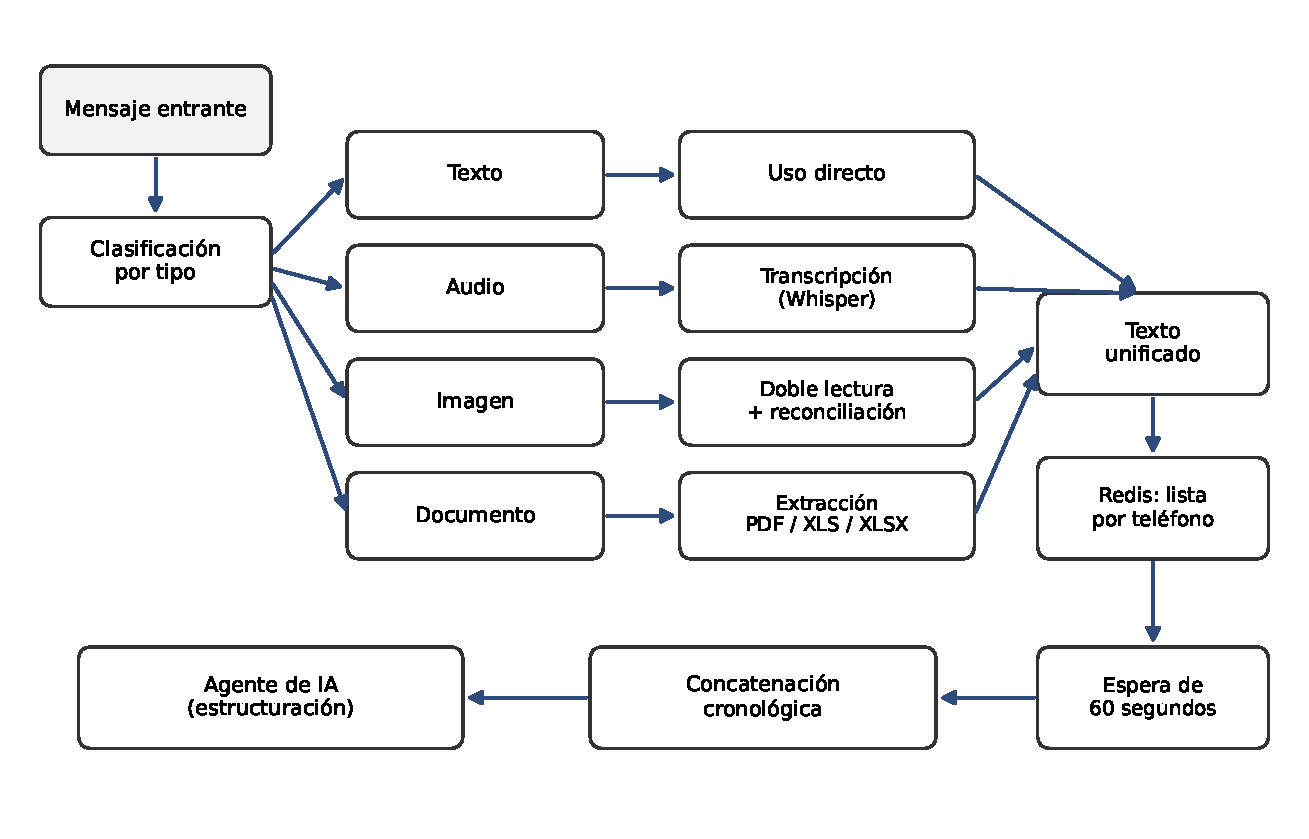
\includegraphics[width=\textwidth]{Figures/flujo_captura.pdf}
  \caption{Procesamiento de la capa de captura, desde el mensaje entrante hasta el texto agrupado.}
  \label{fig:flujo_captura}
\end{figure}

Los mensajes de texto se emplean de forma directa. Los mensajes de voz y las imágenes requieren un paso previo de descarga: la pasarela entrega el contenido multimedia codificado en base64, que luego se convierte en un archivo binario antes de enviarlo al modelo correspondiente. Los mensajes de voz se transcriben con el servicio de transcripción de OpenAI. Los documentos adjuntos se derivan a una rama específica, que reconoce el formato y extrae su contenido mediante los nodos de extracción de PDF y de planillas de cálculo.

El tratamiento de las imágenes constituye el caso más elaborado. La imagen se envía en paralelo a dos modelos de proveedores distintos, GPT-4o de OpenAI y Claude Sonnet de Anthropic. Ambas lecturas se combinan y se entregan a un tercer modelo, que las compara, corrige las diferencias y devuelve una transcripción única.

La instrucción entregada a los modelos de visión no se limita a transcribir el texto visible. Incorpora reglas del dominio que surgieron de la operación real. La más relevante indica conservar la estructura de las tablas y descartar las filas cuya cantidad pedida sea cero. Esa regla resolvió un caso concreto: algunos clientes mayoristas envían una planilla con el catálogo completo del comercio y completan solo unas pocas filas. Sin esa instrucción, el modelo transcribía el listado íntegro y el agente generaba un pedido con decenas de productos no solicitados.

\subsection{Agrupación de mensajes fragmentados}
\label{subsec:agrupacion}

El problema más relevante de esta capa no es la interpretación de un mensaje, sino la determinación de dónde termina un pedido. En el uso real, un cliente rara vez envía su pedido en un único mensaje. Lo habitual es una secuencia de mensajes cortos, con mezcla de texto y audio, enviados en el transcurso de un minuto. Si el sistema procesara cada mensaje por separado, generaría varios pedidos incompletos en lugar de uno correcto.

La solución adoptada consiste en un mecanismo de agrupación por ventana temporal, implementado sobre Redis. Cada texto obtenido se agrega al final de una lista cuya clave es el teléfono del cliente. A continuación, el flujo espera un tiempo determinado. Vencido ese plazo, recupera la lista completa, descarta las entradas inválidas, ordena los elementos por su marca temporal y los concatena en un texto único. La lista se elimina luego para dejar la sesión limpia. Los mensajes que llegan durante la espera se acumulan en la misma lista y quedan incluidos en la agrupación, sin disparar un procesamiento adicional.

La elección de Redis para este mecanismo responde a la naturaleza de los datos involucrados. Se trata de información de vida corta, con alta frecuencia de escritura y lectura, cuya pérdida ante una falla no compromete la operación del negocio. La base relacional se reservó para los datos que sí deben persistir y auditarse.

La ventana se fijó en sesenta segundos. El valor no se eligió a partir del comportamiento de los clientes, sino del tiempo de procesamiento del propio sistema: el intervalo entre el ingreso de un mensaje y la finalización de su procesamiento por los agentes resultó cercano al minuto. Una ventana menor habría cerrado la agrupación antes de que los mensajes previos terminaran de procesarse, con el riesgo de fragmentar el pedido. El valor adoptado constituye entonces una cota conservadora, alineada con la latencia observada. La reducción de ese tiempo de procesamiento permitiría acortar la ventana y, con ella, el tiempo total de respuesta del sistema. Esa optimización se plantea como línea de trabajo futuro en el capítulo \ref{Chapter5}.

%----------------------------------------------------------------------------------------
%	SECTION 3
%----------------------------------------------------------------------------------------

\section{Capa de red y comunicaciones}
\label{sec:capa_red}

En la figura \ref{fig:topologia_despliegue} se presenta la topología de despliegue del sistema, con los servicios contenerizados del servidor virtual y los componentes instalados en el comercio.

\begin{figure}[htbp]
  \centering
  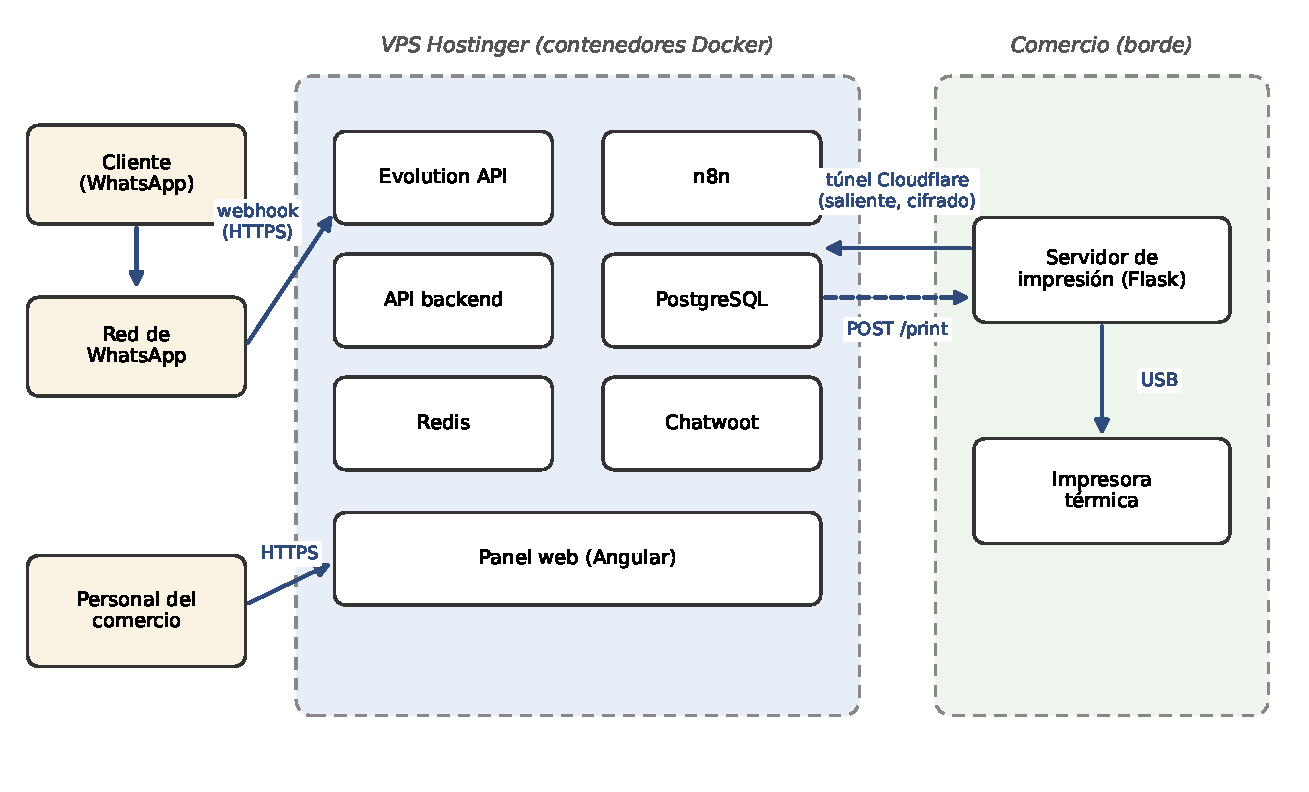
\includegraphics[width=\textwidth]{Figures/topologia_despliegue.pdf}
  \caption{Topología de despliegue del sistema.}
  \label{fig:topologia_despliegue}
\end{figure}

\subsection{Tramos de comunicación}
\label{subsec:tramos}

La conectividad del sistema comprende tres tramos con características distintas.

El primero es el tramo de entrada. La pasarela Evolution API, alojada en el servidor virtual, mantiene la vinculación con la red de WhatsApp y notifica cada mensaje al flujo de n8n mediante peticiones HTTPS, la variante cifrada de HTTP.

El segundo es el tramo interno de la nube. Los servicios contenerizados se comunican entre sí dentro del mismo servidor: el flujo de n8n consulta el catálogo a la API, la API accede a PostgreSQL, y el panel web consume los mismos recursos de la API que utiliza el flujo. Junto a estos servicios opera Chatwoot, una plataforma de gestión de conversaciones que centraliza la bandeja de entrada de WhatsApp. Su integración permite que el personal acceda desde el panel al hilo original de la conversación que dio origen a un pedido, lo que resulta útil ante una interpretación dudosa.

El tercero es el tramo entre la nube y el borde, resuelto mediante el túnel de Cloudflare.

\subsection{Vinculación con el nodo de borde}
\label{subsec:tunel}

La decisión de diseño más relevante de esta capa es el sentido en que se establece la conexión con el comercio. En lugar de exponer el servidor local a Internet mediante la apertura de puertos en el enrutador del negocio, el túnel se establece con una conexión saliente cifrada iniciada desde el propio nodo de borde.

Esta elección tiene tres consecuencias prácticas. La instalación no requiere configurar el equipamiento de red del local, condición decisiva en un comercio sin personal técnico. La red interna del negocio no queda accesible desde el exterior, lo que reduce la superficie de ataque. Y el vínculo se restablece de forma automática tras una interrupción, sin intervención manual.

\subsection{Formato de los mensajes intercambiados}
\label{subsec:payloads}

Los datos que circulan entre los componentes se serializan en formato JSON (del inglés, \textit{JavaScript Object Notation}). El agente de inteligencia artificial produce una estructura fija, que constituye el contrato interno del sistema. El código \ref{lst:pedido_json} muestra su formato.

\begin{lstlisting}[caption={Estructura del pedido devuelto por el agente de interpretación.}, label={lst:pedido_json}]
{
  "is_order": true,
  "items": [
    { "nombre": "Papa", "cantidad": 2, "unidad": "kg" }
  ],
  "aclaraciones": "bien lavadas",
  "productos_no_encontrados": []
}
\end{lstlisting}

El campo \code{is\_order} permite descartar los mensajes que no constituyen un pedido, como saludos o consultas de precio. El campo \code{items} contiene los productos reconocidos, con la denominación exacta del catálogo. El campo \code{aclaraciones} recoge las instrucciones y observaciones del cliente. El campo \code{productos\_no\_\allowbreak encontrados} registra las menciones que no pudieron asociarse a ningún artículo del catálogo, en lugar de descartarlas en silencio. Esta última decisión resultó importante para la trazabilidad: un producto solicitado y no reconocido queda registrado y visible para el personal, en vez de desaparecer del pedido.

El segundo contrato relevante es el del servidor de impresión. El código \ref{lst:print_json} muestra la petición que la API envía al nodo de borde.

\begin{lstlisting}[caption={Petición de impresión enviada al servidor local.}, label={lst:print_json}]
POST /print
X-Printer-Token: <token>

{
  "text": "PEDIDO\n...",
  "printer_name": "Hasar_USB",
  "cut": true,
  "text_size": "double_width"
}
\end{lstlisting}

El campo \code{text} contiene el ticket ya compuesto. Los campos restantes controlan el destino y el formato de impresión: el nombre de la impresora instalada, el corte automático del papel al finalizar y el tamaño de la tipografía. De manera alternativa, la petición admite una dirección IP y un puerto, para el caso en que la impresora se conecte por red. Esa previsión permite trasladar la impresora dentro del local sin modificar el código, tal como se anticipó en el capítulo \ref{Chapter2}.

El servidor de impresión resuelve el envío según la plataforma sobre la que se ejecuta. En Windows utiliza la interfaz de impresión del sistema operativo en modo directo, lo que evita que el controlador reinterprete el contenido y preserva los comandos ESC/POS. En sistemas Linux delega en el sistema de impresión estándar, y ante una impresora de red abre una conexión directa al puerto correspondiente. Esta triple implementación permitió desarrollar y ensayar el componente fuera del entorno del comercio.

%----------------------------------------------------------------------------------------
%	SECTION 4
%----------------------------------------------------------------------------------------

\section{Capa de aplicación y procesamiento}
\label{sec:capa_aplicacion}

Esta capa concentra la interpretación de los pedidos, su validación, la resolución de precios y su persistencia. Es la de mayor complejidad lógica y la que resuelve el problema central del trabajo.

\subsection{Interpretación mediante agentes de inteligencia artificial}
\label{subsec:interpretacion_ia}

La interpretación se implementó como un agente de inteligencia artificial orquestado en n8n. El agente recibe cuatro insumos: el texto agrupado del cliente, sus datos de contacto, el catálogo vigente de productos y la lista de unidades admitidas. Los dos últimos no están fijados en el flujo, sino que se consultan a la API en cada ejecución mediante recursos internos previstos para ese fin. Esta decisión evita la duplicación del catálogo: el personal lo administra desde el panel y el agente siempre opera con la versión actualizada.

El agente cuenta además con memoria de ventana, cuya clave de sesión se construye a partir del teléfono del cliente. De este modo, cada conversación mantiene su contexto de forma independiente.

El comportamiento del agente se define mediante un mensaje de sistema, es decir, la instrucción permanente que delimita su rol y sus reglas antes de recibir cada mensaje del cliente. Su redacción constituyó una parte sustancial del desarrollo, porque de ella dependen tanto la calidad de la interpretación como la estabilidad del formato de salida. El código \ref{lst:prompt_agente} reproduce sus fragmentos más representativos.

\begin{lstlisting}[caption={Fragmentos del mensaje de sistema del agente de interpretación.}, label={lst:prompt_agente}]
# ROL
Sos un asistente para una verduleria. Tu unica tarea es:
1. Determinar si el mensaje del cliente es un pedido de compra.
2. Extraer los productos, cantidades y unidades solicitados.

# CATALOGO
- Para el campo `nombre` en cada item, usa exactamente el nombre
  del catalogo.
- Si el cliente menciona un producto que no esta en el catalogo,
  ponelo en `productos_no_encontrados` (no en `items`).
- Si el cliente usa un apodo o abreviatura que corresponde a un
  producto del catalogo, usa el nombre del catalogo.

# SALIDA
Devolve unicamente el JSON, sin texto adicional ni marcado.
\end{lstlisting}

Tres criterios guiaron esa redacción. El primero es la delimitación estricta del rol, que evita que el agente responda consultas ajenas al pedido. El segundo es la restricción del formato de salida, indispensable para consumir la respuesta de forma programática. El tercero es el tratamiento explícito de los casos ambiguos, que impide que el modelo complete por su cuenta la información faltante.

\subsection{Normalización semántica de productos}
\label{subsec:normalizacion}

Un problema específico del dominio es la variabilidad con que los clientes nombran un mismo producto. Las denominaciones llegan en plural o singular, con diminutivos, con abreviaturas o con errores de tipeo. El sistema debe asociarlas al artículo correcto del catálogo del comercio.

La normalización se resolvió dentro del propio agente, mediante la entrega del catálogo completo como contexto y una instrucción explícita de correspondencia tolerante a variantes. El agente debe utilizar la denominación exacta del catálogo en el campo de salida. Cuando una mención no admite correspondencia razonable, se deriva al campo de productos no encontrados.

Se consideró como alternativa una normalización previa por reglas o por similitud de cadenas. Esa opción se descartó por dos razones. La primera es que las reglas exigen mantenimiento manual ante cada producto nuevo o cada variante no prevista. La segunda es que la similitud de cadenas resuelve mal los casos en que la diferencia es semántica y no ortográfica, como una denominación regional que no comparte raíz con el nombre del catálogo. La estrategia adoptada traslada esa responsabilidad al modelo, que dispone del catálogo completo y del contexto del mensaje.

\subsection{Recursos de la interfaz de programación}
\label{subsec:api}

La API se organizó por recursos, con un prefijo común y un archivo de rutas por entidad. En la tabla \ref{tab:endpoints} se resumen los grupos de recursos y su mecanismo de acceso.

\begin{table}[htbp]
  \centering
  \caption{Grupos de recursos de la interfaz de programación.}
  \label{tab:endpoints}
  \small
  \begin{tabular}{l l l}
    \toprule
    \textbf{Recurso}         & \textbf{Función}             & \textbf{Acceso}             \\
    \midrule
    \code{/auth}             & Autenticación de personas    & Público                     \\
    \code{/pedidos}          & Creación, consulta y edición & Clave de servicio o testigo \\
    \code{/productos}        & Catálogo de productos        & Testigo (catálogo: clave)   \\
    \code{/unidades}         & Unidades de medida           & Testigo (catálogo: clave)   \\
    \code{/categorias}       & Categorías de productos      & Testigo, rol administrador  \\
    \code{/clientes}         & Clientes y listas de precios & Testigo                     \\
    \code{/precios\_default} & Precios generales            & Testigo                     \\
    \code{/print-logs}       & Historial de impresiones     & Testigo                     \\
    \code{/metricas}         & Indicadores de operación     & Testigo                     \\
    \code{/usuarios}         & Usuarios del sistema         & Testigo, rol administrador  \\
    \bottomrule
  \end{tabular}
\end{table}

La creación de un pedido desde el flujo automático y su creación desde el panel se resolvieron con recursos distintos, aunque compartan la lógica de persistencia. La separación responde a que difieren en su origen, en su mecanismo de autenticación y en la validación aplicada: el flujo entrega productos ya normalizados por el agente, mientras que el panel recibe datos ingresados por una persona.

\subsection{Modelo de datos}
\label{subsec:modelo_datos}

La persistencia se resolvió sobre PostgreSQL, con acceso mediante el ORM Prisma. El esquema se controla por migraciones versionadas, lo que permite reproducir la estructura de la base en cualquier entorno. En la figura \ref{fig:der} se presenta el diagrama entidad-relación con las entidades principales.

\begin{figure}[htbp]
  \centering
  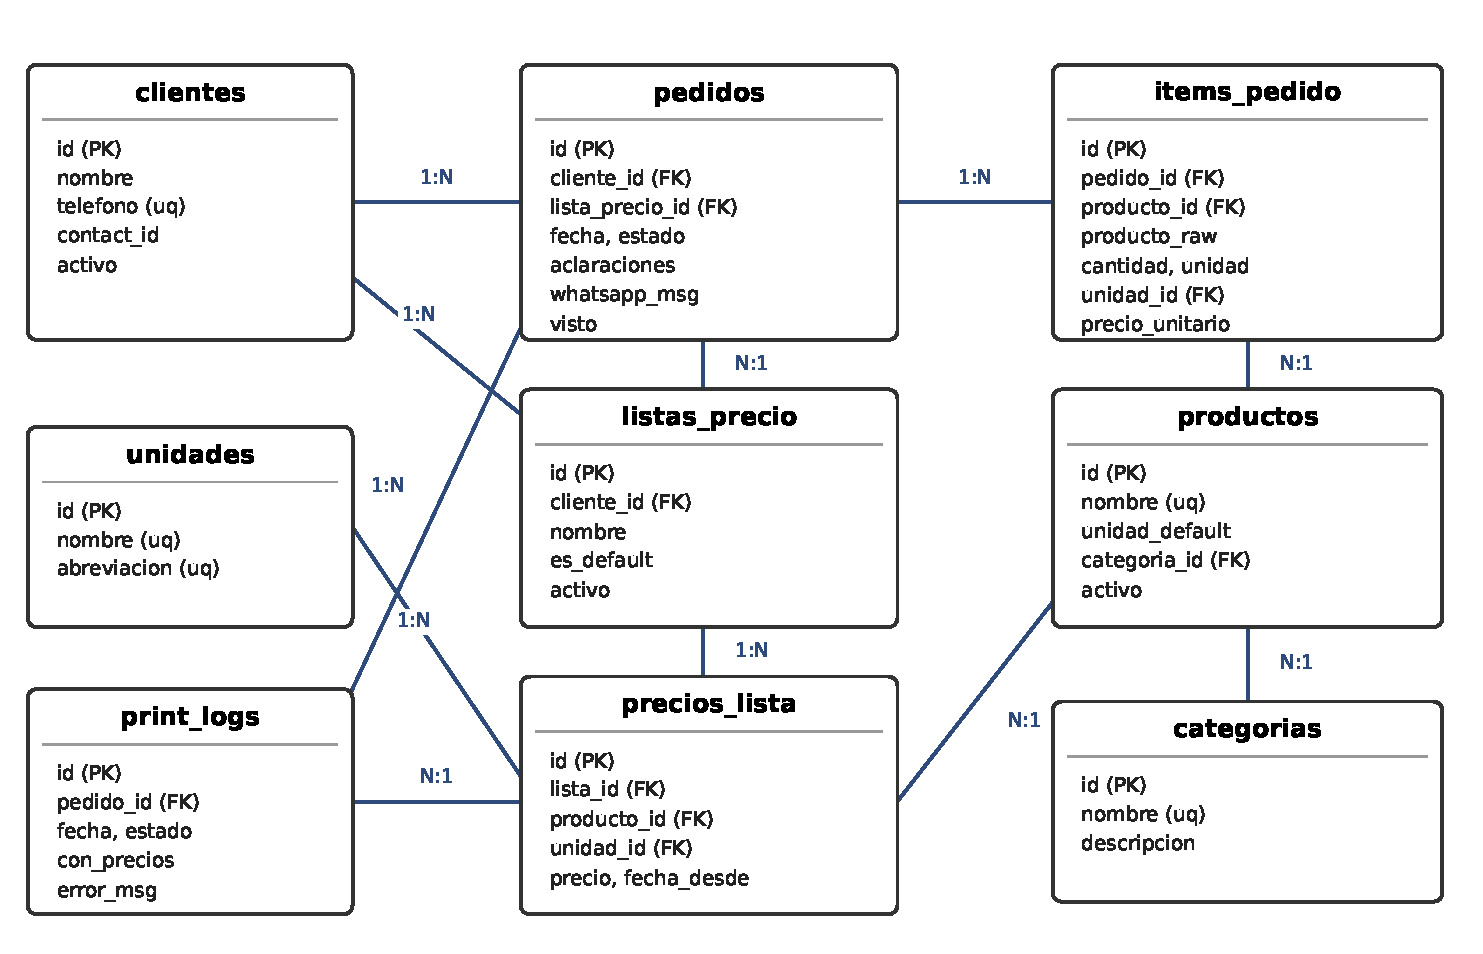
\includegraphics[width=\textwidth]{Figures/der_base_datos.pdf}
  \caption{Diagrama entidad-relación de la base de datos.}
  \label{fig:der}
\end{figure}

El núcleo del modelo lo constituyen las entidades \code{clientes}, \code{pedidos} e \code{items\_\allowbreak pedido}. Un cliente se identifica por su teléfono, con restricción de unicidad, y acumula sus pedidos. Cada pedido registra la fecha, el estado, las aclaraciones y el mensaje original recibido por WhatsApp. Este último campo resulta clave para la trazabilidad, ya que permite contrastar el pedido estructurado contra el texto que le dio origen.

La entidad \code{items\_pedido} presenta una particularidad de diseño. Junto a la referencia al producto del catálogo conserva un campo con la denominación original empleada por el cliente. Cuando la referencia al catálogo queda vacía, el ítem corresponde a un producto no reconocido. Esos ítems no se descartan: se conservan, se imprimen en una sección separada del ticket y se destacan visualmente en el panel para que el personal decida cómo proceder.

El estado del pedido se modeló como una enumeración con cuatro valores: recibido, en preparación, listo y entregado. La enumeración impide que la base admita estados no previstos y ordena el recorrido operativo del pedido dentro del comercio.

El modelo contempla además dos operaciones propias del uso real. La primera es la fusión de pedidos: cuando un cliente envía un pedido complementario poco después del primero, el personal puede unificarlos desde el panel. El modelo conserva la referencia al pedido resultante y la marca temporal de la operación, lo que permite deshacerla sin pérdida de información. La segunda es la marca de pedido visto, que distingue los pedidos ya revisados por el personal de los que aún esperan atención.

\subsection{Resolución de precios}
\label{subsec:precios}

La gestión de precios responde a una característica del negocio: no todos los clientes pagan lo mismo. El comercio atiende tanto a consumidores finales como a otros comercios, con condiciones diferenciadas.

El modelo resuelve esa necesidad mediante listas de precios. Cada cliente puede tener varias listas, y una de ellas se designa como predeterminada. El precio de un ítem se resuelve por orden de prioridad: primero la lista indicada de forma explícita en el pedido, luego la lista predeterminada del cliente y, por último, el precio general del catálogo. Los precios incorporan además vigencia temporal, con fechas de inicio y de fin, lo que permite conservar el histórico sin perder el valor aplicado en cada momento.

Un diseño alternativo, con un único precio por cliente y producto, habría resultado más simple. Se descartó porque impide representar acuerdos comerciales distintos para un mismo cliente, como una condición mayorista y otra minorista, y porque no conserva el histórico de precios necesario para las métricas de facturación.

\subsection{Generación del ticket}
\label{subsec:ticket}

El ticket no se almacena en la base de datos, sino que se compone en el momento de la impresión a partir de los ítems del pedido y de sus aclaraciones. Esta decisión evita la duplicación de información y garantiza que una reimpresión refleje el estado actual del pedido, incluidas las correcciones realizadas por el personal.

La impresión admite dos variantes, con precios y sin precios. El flujo automático imprime sin precios, porque el ticket cumple allí la función de orden de armado. Desde el panel, en cambio, el personal elige la variante al momento de imprimir, según entregue el comprobante al cliente o lo destine al armado interno.

Cada intento de impresión se registra en una entidad específica, con su resultado, la variante utilizada y el mensaje de error en caso de falla. Ese registro cumple dos funciones: permite auditar qué se imprimió y cuándo, y habilita el seguimiento de los errores hasta su resolución. Los pedidos con impresión fallida se destacan en el panel y permanecen señalados hasta que el personal los marca como resueltos, de modo que una falla de la impresora no derive en un pedido sin atender.

%----------------------------------------------------------------------------------------
%	SECTION 5
%----------------------------------------------------------------------------------------

\section{Interfaz de usuario y visualización}
\label{sec:interfaz}

El sistema presenta dos interfaces hacia el personal del comercio: el ticket impreso y el panel web de control.

\subsection{El ticket impreso}
\label{subsec:ticket_impreso}

El ticket es la salida física del sistema y el insumo directo para el armado del pedido. Su formato es fijo. Incluye un encabezado con los datos del cliente, la lista de productos con cantidades y unidades, una sección separada para los productos no reconocidos, un espacio para las aclaraciones y la fecha y hora del pedido. En la figura \ref{fig:ticket} se muestra un ticket generado por el sistema.

\begin{figure}[htbp]
  \centering
  % [PENDIENTE: reemplazar por la fotografía del ticket impreso, con datos de ejemplo.]
  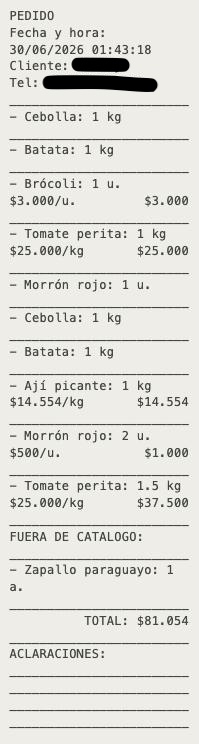
\includegraphics[width=0.45\textwidth]{Figures/ticket_impreso.jpeg}
  \caption{Ticket generado por el sistema e impreso en el comercio.}
  \label{fig:ticket}
\end{figure}

El diseño del ticket estuvo condicionado por el medio. El ancho útil del papel es de ochenta milímetros, lo que limita la cantidad de caracteres por línea y obliga a priorizar la información. Por ese motivo, el servidor de impresión admite distintos tamaños de tipografía, que se aplican mediante comandos ESC/POS. Los datos que el personal necesita leer a distancia, en particular el nombre del cliente, se imprimen en tamaño ampliado, mientras que el detalle de los productos se mantiene en tamaño normal para aprovechar el ancho disponible.

\subsection{El panel web de control}
\label{subsec:panel}

El panel se desarrolló con Angular y la biblioteca de componentes Angular Material. Concentra la operación diaria y la administración del sistema. El acceso está protegido por autenticación, y las vistas de administración quedan restringidas según el rol de la persona que ingresa.

\subsubsection{Tablero principal}

El tablero es la vista de entrada al sistema y resume el estado de la operación del día. En la figura \ref{fig:panel_dashboard} se presenta esa vista.

\begin{figure}[htbp]
  \centering
  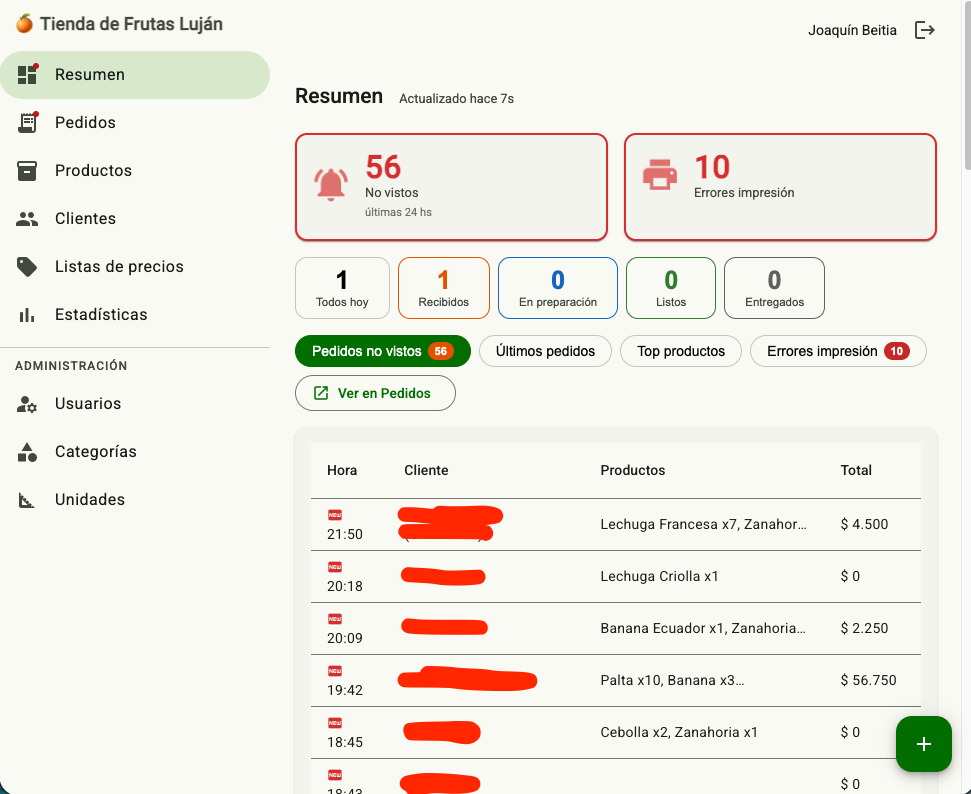
\includegraphics[width=\textwidth]{Figures/panel_dashboard.png}
  \caption{Tablero principal del panel de control.}
  \label{fig:panel_dashboard}
\end{figure}

El tablero agrupa cuatro bloques de información: los pedidos aún no revisados por el personal, los pedidos recibidos en los últimos minutos, los productos más solicitados en el día y los pedidos con errores de impresión pendientes de resolución. Cada bloque enlaza con la vista de pedidos, con los filtros ya aplicados, de modo que una alerta deriva de forma directa en la acción correspondiente.

\subsubsection{Gestión de pedidos}

La vista de pedidos es la de mayor uso durante la jornada. Permite filtrar por estado, por rango de fechas, por pedidos no vistos y por errores de impresión. En la figura \ref{fig:panel_pedidos} se muestra el listado.

\begin{figure}[htbp]
  \centering
  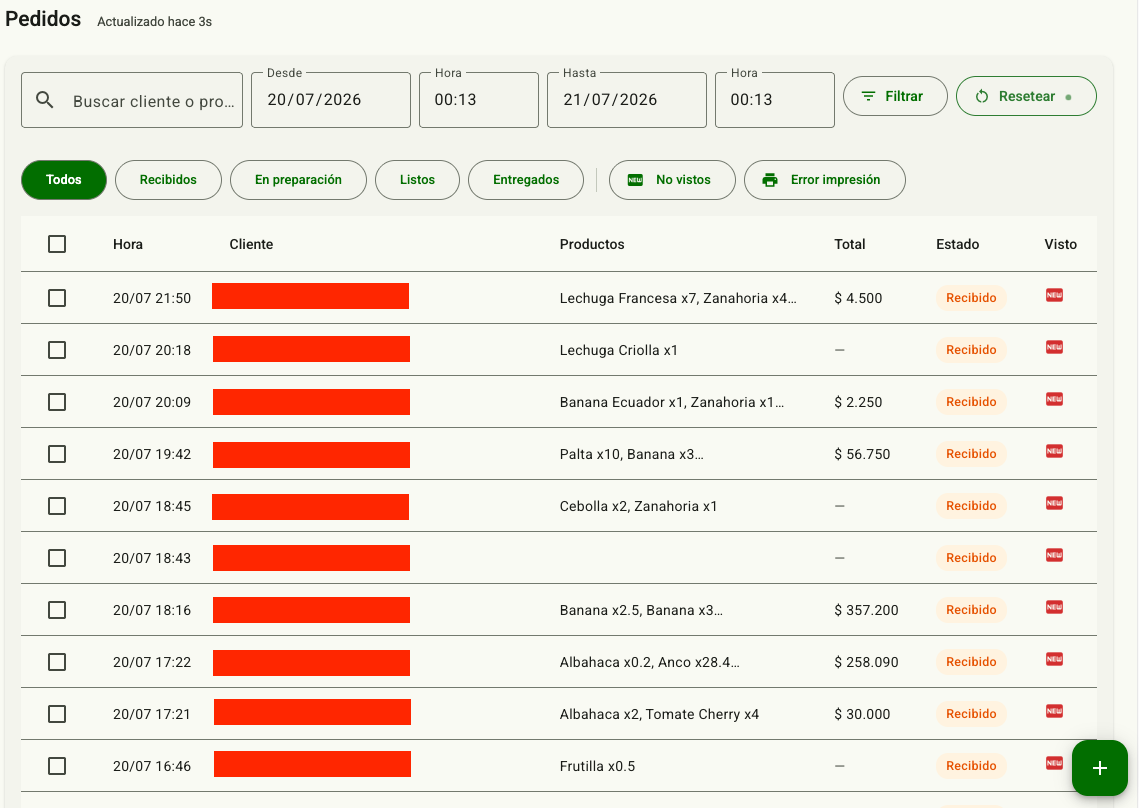
\includegraphics[width=\textwidth]{Figures/panel_pedidos.png}
  \caption{Listado de pedidos con sus filtros de búsqueda.}
  \label{fig:panel_pedidos}
\end{figure}

El listado admite operaciones sobre varios pedidos a la vez, como el cambio de estado o la marca de revisado, pensadas para los momentos de mayor demanda. El detalle de cada pedido se abre en un diálogo que concentra la operación individual, según se observa en la figura \ref{fig:panel_detalle}.

\begin{figure}[htbp]
  \centering
  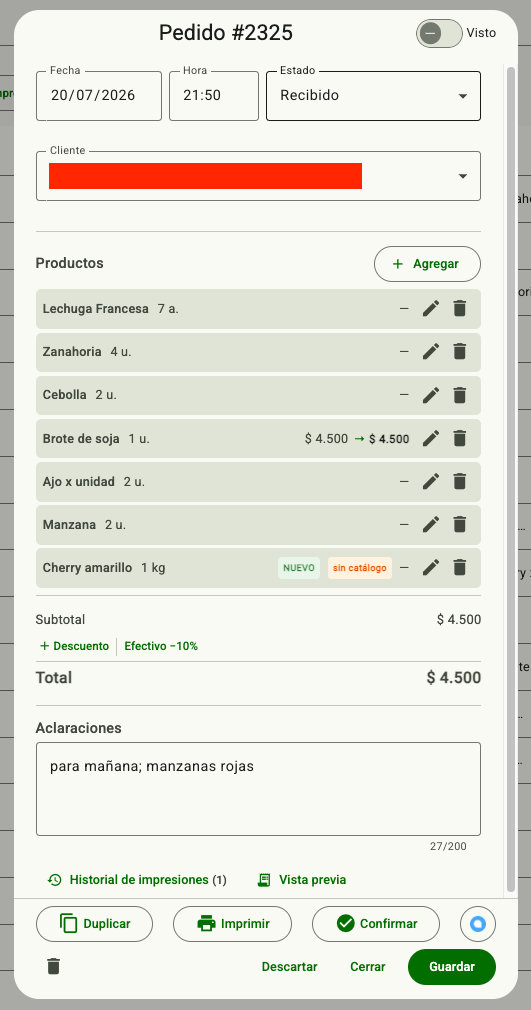
\includegraphics[width=0.55\textwidth]{Figures/panel_detalle_pedido.png}
  \caption{Detalle de un pedido, con edición de ítems y acceso al mensaje original.}
  \label{fig:panel_detalle}
\end{figure}

Desde ese diálogo, el personal puede corregir las cantidades y las unidades, agregar o quitar ítems, consultar el mensaje original recibido por WhatsApp, acceder al hilo de la conversación e imprimir o reimprimir el pedido. Los ítems que no pudieron asociarse al catálogo se destacan de forma visual, lo que dirige la atención del personal hacia los casos que requieren decisión.

\subsubsection{Administración del catálogo y de los precios}

El catálogo de productos, sus categorías y las unidades de medida se administran desde el panel. Esta gestión resulta crítica para el funcionamiento del sistema, ya que el catálogo es el insumo que el agente utiliza para normalizar las denominaciones. Un producto ausente del catálogo se traduce de inmediato en ítems no reconocidos en los pedidos.

\begin{figure}[htbp]
  \centering
  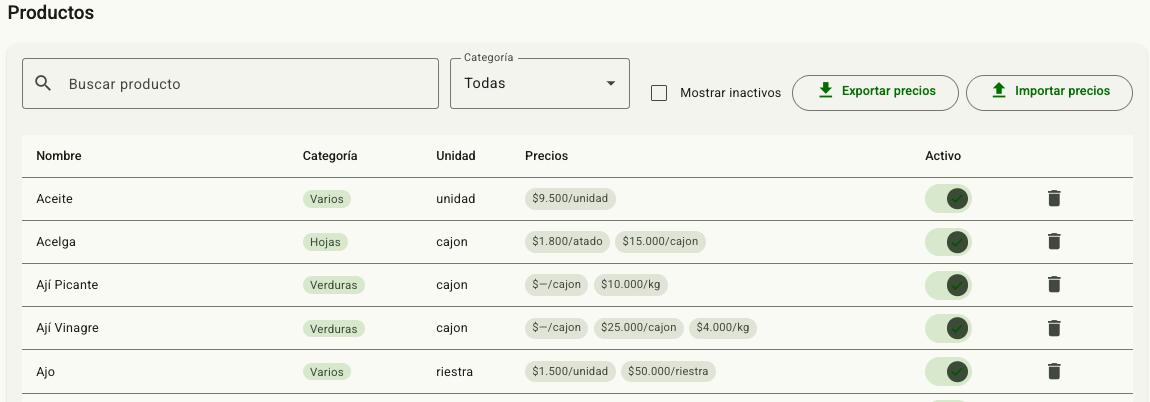
\includegraphics[width=\textwidth]{Figures/panel_productos.png}
  \caption{Administración del catálogo de productos.}
  \label{fig:panel_productos}
\end{figure}

La administración de precios se resolvió en una vista específica, con el listado de listas del cliente a un lado y la tabla de precios editable al otro. En la figura \ref{fig:panel_precios} se presenta esa vista.

\begin{figure}[htbp]
  \centering
  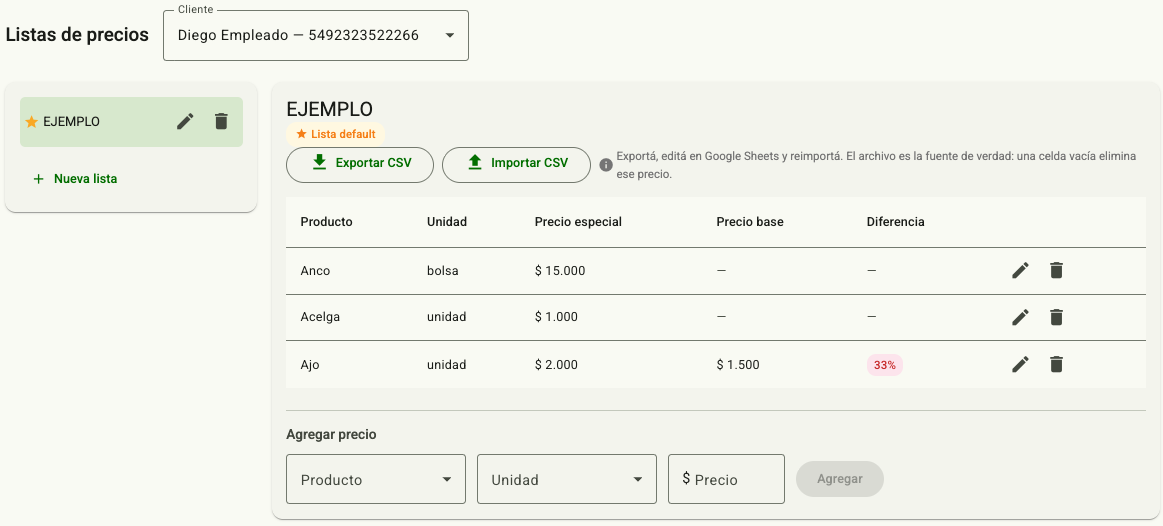
\includegraphics[width=\textwidth]{Figures/panel_listas_precios.png}
  \caption{Administración de las listas de precios de un cliente.}
  \label{fig:panel_precios}
\end{figure}

\subsubsection{Métricas de operación}

Las métricas se representan con la biblioteca Chart.js. La vista incluye el tráfico de pedidos por día y hora, la evolución de la facturación por producto y la distribución por categoría. En la figura \ref{fig:panel_estadisticas} se muestra esa vista.

\begin{figure}[htbp]
  \centering
  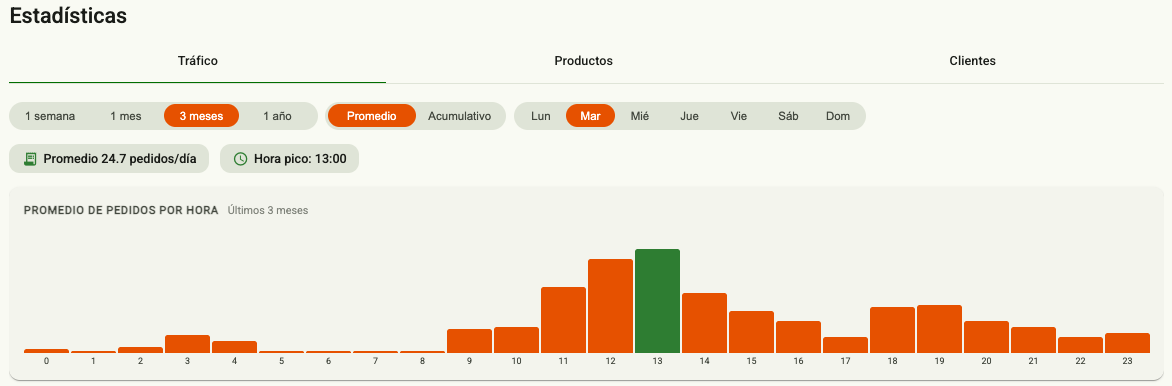
\includegraphics[width=\textwidth]{Figures/panel_estadisticas.png}
  \caption{Vista de métricas de operación del comercio.}
  \label{fig:panel_estadisticas}
\end{figure}

La consulta admite distintos rangos temporales, y la granularidad de la serie se ajusta de forma automática al rango solicitado: diaria hasta una semana, semanal hasta tres meses y mensual para períodos mayores. Este ajuste evita gráficos ilegibles por exceso de puntos. El tráfico por día y hora resultó de utilidad directa para el negocio, ya que expone los momentos de mayor demanda y permite anticipar la asignación de personal.

%----------------------------------------------------------------------------------------
%	SECTION 6
%----------------------------------------------------------------------------------------

\vspace{50em}
\section{Seguridad del sistema}
\label{sec:seguridad}

La seguridad se abordó en tres frentes: el control de acceso, la protección de las comunicaciones y la integridad de los datos.

\subsection{Autenticación y control de acceso}
\label{subsec:autenticacion}

El sistema distingue dos tipos de consumidores, con mecanismos de autenticación distintos. Las personas acceden al panel con credenciales y obtienen un testigo de sesión. Los servicios internos, como el flujo de n8n, no disponen de una sesión de usuario y se autentican con una clave de servicio. En la figura \ref{fig:auth} se representan ambos mecanismos.

\begin{figure}[htbp]
  \centering
  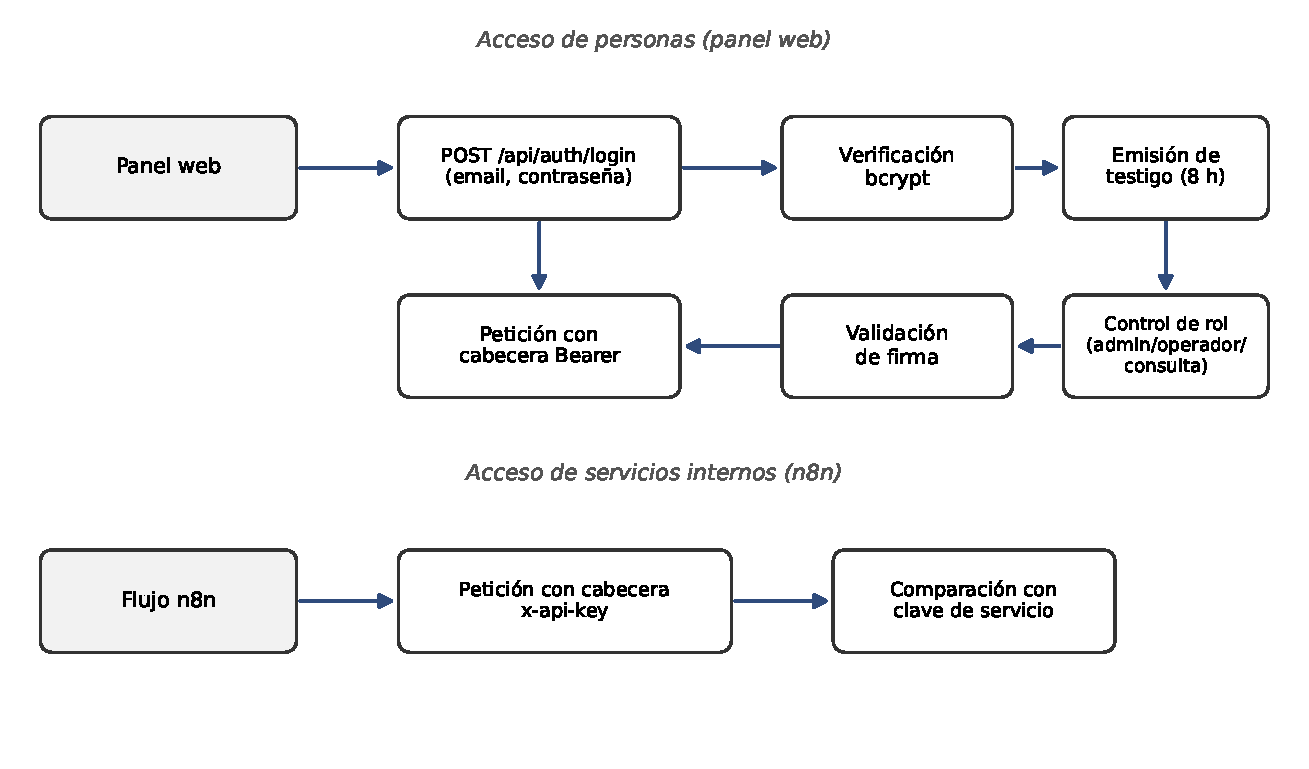
\includegraphics[width=\textwidth]{Figures/flujo_autenticacion.pdf}
  \caption{Mecanismos de autenticación para personas y para servicios internos.}
  \label{fig:auth}
\end{figure}

Las contraseñas se almacenan cifradas mediante una función de derivación diseñada para ese fin, de modo que la base no conserva las claves en texto plano. Tras una validación exitosa, el sistema emite un testigo firmado con vigencia de ocho horas, que el panel adjunta en cada petición posterior. La vigencia se ajustó a la duración de una jornada comercial, lo que evita tanto la reautenticación durante el turno como la persistencia indefinida de una sesión abierta.

La autorización se implementó por roles. El sistema define tres: administrador, con acceso total; operador, restringido a la operación de pedidos; y consulta, limitado a la lectura. La verificación se resuelve con un componente intermedio que valida el rol antes de ejecutar cada operación, lo que centraliza la regla y evita repetirla en cada recurso. El panel replica esa restricción en sus rutas, de modo que las vistas de administración no resultan accesibles para los roles que no corresponden.

Los recursos internos, como la consulta del catálogo y la creación de pedidos desde el flujo, admiten únicamente la clave de servicio. El recurso de impresión constituye una excepción deliberada, ya que acepta ambas formas de autenticación: la clave de servicio para la impresión automática y el testigo de sesión para la reimpresión desde el panel.

\subsection{Protección de las comunicaciones}
\label{subsec:proteccion_comunicaciones}

Todo el tráfico externo circula cifrado. La pasarela de mensajería entrega los mensajes por HTTPS y el vínculo entre la nube y el borde se resuelve mediante el túnel descripto en la sección \ref{subsec:tunel}, cuya conexión saliente cifrada evita exponer puertos entrantes en la red del comercio. El servidor de impresión exige, además, un testigo propio en cada petición, de modo que la sola llegada al servicio no habilita la impresión.

\subsection{Gestión de credenciales e integridad de los datos}
\label{subsec:credenciales}

Las credenciales de los servicios externos y las claves de firma se gestionan mediante variables de entorno, fuera del código fuente. Los archivos que las contienen quedan excluidos del control de versiones, y el repositorio conserva únicamente valores de ejemplo. Este criterio evita que una credencial operativa quede registrada en el historial del repositorio.

En cuanto a la integridad, el modelo de datos define restricciones de unicidad sobre los campos que identifican a clientes, productos y unidades, y relaciones con integridad referencial entre las entidades. La eliminación de un pedido arrastra sus ítems y sus registros de impresión, lo que evita la persistencia de datos huérfanos. Redis se reservó de manera estricta para información temporal, de modo que una falla en la capa en memoria no compromete los registros del negocio.
% !TEX root = ../memorianueva.tex
% Chapter 4

\chapter{Ensayos y resultados} % Main chapter title

\label{Chapter4} % Para referenciar este capítulo: \ref{Chapter4}

En el presente capítulo se describen las pruebas realizadas sobre el sistema y los resultados obtenidos. Se presenta primero el plan de ensayos, con su metodología, sus instrumentos de medición y sus criterios de evaluación. Luego se exponen los ensayos de conectividad y comunicación, los de la capa de aplicación y los de integración extremo a extremo. El capítulo cierra con el análisis de los resultados, las limitaciones detectadas y las mejoras que se desprenden de ellas.

%----------------------------------------------------------------------------------------
%	SECTION 1
%----------------------------------------------------------------------------------------

\section{Plan de ensayos}
\label{sec:plan_ensayos}

El plan de ensayos se organizó en dos niveles complementarios. El primero corresponde a la verificación y reúne las pruebas orientadas a comprobar que cada componente fue construido de acuerdo con lo especificado. El segundo corresponde a la validación y reúne las pruebas ejecutadas sobre el sistema en operación real en el comercio, orientadas a comprobar que la solución resuelve el problema planteado.

\subsection{Alcance y ventanas de medición}
\label{subsec:alcance_medicion}

La condición particular de este trabajo es que el sistema se desplegó en producción y operó de forma continua durante el período de evaluación. Esa circunstancia permitió sustituir buena parte de los ensayos de laboratorio por mediciones sobre la operación real, con un volumen de casos muy superior al que habría aportado un banco de pruebas construido para la ocasión.

El sistema entró en operación el 1 de junio de 2026 y el primer pedido quedó registrado el 4 de junio. Sobre la ventana comprendida entre esa fecha y el 17 de agosto de 2026 se procesaron 3871 pedidos de 202 clientes, con un total de 29\,457 ítems y un promedio de 7,61 ítems por pedido.

Las mediciones no cubren todas un mismo intervalo, ya que cada subsistema conserva su información durante un lapso distinto.

En la tabla \ref{tab:ventanas} se detallan las tres ventanas empleadas y el motivo de su extensión.

\begin{table}[H]
    \centering
    \caption{Ventanas de medición empleadas en los ensayos.}
    \label{tab:ventanas}
    \begin{tabular}{L{4.9cm} L{3.1cm} c L{3.0cm}}
        \toprule
        \textbf{Aspecto medido}             & \textbf{Período}    & \textbf{Días} & \textbf{Limitación}                     \\
        \midrule
        Captura e interpretación de pedidos & 04/06 al 17/08/2026 & 75            & Inicio de la operación                  \\
        Impresión automática en el borde    & 29/06 al 17/08/2026 & 50            & Habilitación de la impresión automática \\
        Ejecuciones de la orquestación      & 04/08 al 17/08/2026 & 14            & Purga automática de ejecuciones         \\
        \bottomrule
    \end{tabular}
\end{table}

La diferencia entre la primera y la segunda ventana obedece a la puesta en marcha escalonada. Durante las cuatro primeras semanas la capa de captura e interpretación operó con el volumen completo de pedidos sin impresora térmica en el comercio, y los resultados se volcaron a un archivo de texto en la nube que el personal consultaba de forma manual. La actuación automática en el borde se habilitó en la semana del 29 de junio, una vez instalada la impresora y verificada la calidad de la interpretación, tras lo cual el volumen se estabilizó por encima de las quinientas operaciones semanales. Diferir la automatización hasta contar con esa evidencia constituyó una medida deliberada de reducción de riesgo operativo.

La tercera ventana responde a una restricción del registro de ejecuciones de la plataforma de orquestación, que conserva las ejecuciones durante 14 días y luego las elimina de forma automática. Sobre ese lapso se registraron 7036 ejecuciones y 789 pedidos.

\subsection{Instrumentos de medición}
\label{subsec:instrumentos}

La medición se apoyó en tres fuentes de información distintas.

La primera es la base de datos relacional del sistema, que registra cada pedido, cada ítem y cada intento de impresión con su marca temporal y su resultado: la tabla \code{print\_logs} conserva el estado de cada operación de impresión, y la ausencia de valor en el campo \code{producto\_id} de \code{items\_pedido} identifica los ítems no vinculados al catálogo. Esta fuente aporta la totalidad de la información de las secciones \ref{sec:ensayos_conectividad} y \ref{sec:ensayos_aplicacion}, aunque conserva el pedido ya estructurado y no el mensaje original.

La segunda es el registro de ejecuciones de la plataforma de orquestación, que conserva el instante de inicio y de finalización de cada flujo junto con su estado final. Esa información permite acotar el tiempo de interpretación, que no queda registrado en la base relacional del sistema.

La tercera es la plataforma de atención vinculada al canal de mensajería, que conserva cada mensaje entrante con su marca temporal, su contacto de origen y el tipo de contenido de sus adjuntos. Esa fuente aporta la única información disponible sobre el formato del mensaje original, dimensión que las dos anteriores no permiten discriminar, y sostiene la auditoría de la subsección \ref{subsec:ensayo_formatos}. Su vinculación con los pedidos no es directa, ya que ambos sistemas no comparten identificadores, y debió reconstruirse por coincidencia del número de contacto y proximidad temporal según el procedimiento que allí se detalla.

\subsection{Estrategia de verificación adoptada}
\label{subsec:estrategia_verificacion}

Los requerimientos de testing previeron la ejecución de pruebas unitarias sobre los módulos de procesamiento e impresión y de pruebas de integración entre los componentes. La revisión del repositorio confirmó que no se implementaron conjuntos de pruebas automatizadas, más allá del archivo de ejemplo que genera el entorno de desarrollo del panel, que no contiene casos de prueba.

En su reemplazo, la verificación se apoyó en la operación real del sistema durante 75 días. Esa estrategia aporta una cobertura de casos superior a la que habría alcanzado un conjunto de pruebas construido para la ocasión, con la variabilidad propia de los mensajes de clientes reales, y permite validar de forma simultánea la integración de todos los componentes. Su limitación es que no detecta regresiones de manera anticipada ni permite aislar la causa de una falla en un componente determinado, motivo por el que la incorporación de pruebas automatizadas se propone como trabajo futuro en el capítulo \ref{Chapter5}.

\subsection{Criterios de evaluación}
\label{subsec:criterios}

La planificación del trabajo definió, para cada requerimiento, un método de verificación y un método de validación, pero no estableció valores numéricos de corte con anterioridad al desarrollo. Los ensayos descriptos en este capítulo son, en consecuencia, de caracterización: se orientan a determinar el comportamiento efectivo del sistema en operación antes que a contrastarlo contra umbrales preestablecidos.

El criterio de aceptación que operó de manera efectiva fue la validación por parte del cliente en el entorno real. El sistema se incorporó a la operación diaria del comercio y permaneció en uso continuo durante todo el período analizado, lo que constituye una forma de aceptación por uso sostenido. En la subsección \ref{subsec:verificacion_requerimientos} se contrasta cada requerimiento contra la evidencia obtenida.

%----------------------------------------------------------------------------------------
%	SECTION 2
%----------------------------------------------------------------------------------------

\section{Ensayos de conectividad y comunicación}
\label{sec:ensayos_conectividad}

Los ensayos de conectividad se orientaron a verificar el vínculo entre la nube y el nodo de borde, que constituye el único punto de contacto entre ambos entornos y, por lo tanto, el eslabón crítico de la cadena. La medición se apoyó en la operación real: cada intento de envío de un ticket hacia el servidor local quedó registrado con su resultado y, en caso de falla, con el mensaje de error devuelto.

\subsection{Confiabilidad del vínculo en operación}
\label{subsec:confiabilidad_vinculo}

El análisis distingue el período de prueba de la impresora del período de operación automática, ya que las condiciones difieren por completo. Durante las cuatro primeras semanas, cuando el comercio aún no contaba con el equipo, se registraron 39 operaciones de impresión, de las que 13 finalizaron con error. Esos casos carecen de valor para evaluar la confiabilidad del vínculo, dado que el destino de la orden no existía.

Durante el período de operación automática, comprendido entre el 29 de junio y el 17 de agosto, se registraron 4334 operaciones de impresión, de las que 22 finalizaron con error, lo que arroja una tasa de fallas del 0,51 por ciento.
En la tabla \ref{tab:errores_conectividad} se detalla la clasificación de los errores del período de operación automática según su mensaje y su origen.

\begin{table}[H]
    \centering
    \caption{Clasificación de los errores registrados durante la operación automática.}
    \label{tab:errores_conectividad}
    \begin{tabular}{l L{6.2cm} c}
        \toprule
        \textbf{Mensaje}  & \textbf{Origen}               & \textbf{Casos} \\
        \midrule
        HTTP 530          & Túnel sin origen alcanzable   & 18             \\
        HTTP 502          & Pasarela intermedia           & 2              \\
        HTTP 520          & Respuesta inválida del origen & 1              \\
        Fallo de conexión & Red entre la nube y el túnel  & 1              \\
        \midrule
        Total             &                               & 22             \\
        \bottomrule
    \end{tabular}
\end{table}

La totalidad de los errores del período de operación automática corresponde a interrupciones del vínculo de comunicación. Los códigos 530 y 520 son emitidos por el proveedor del túnel cuando el extremo local no responde, situación que se produce ante una caída de la conexión a Internet del comercio o ante la detención del proceso en el servidor local. Ningún error se originó en la impresora ni en el formateo del ticket, lo que indica que la actuación física en el borde resultó estable durante todo el período.

Este comportamiento respalda el criterio de distribución del cómputo adoptado en la subsección \ref{subsec:criterio_distribucion}. La única dependencia externa del proceso de impresión es la llegada de la orden desde la nube, y una vez que esa orden alcanza el nodo de borde la operación se completa sin intermediarios.

\subsection{Análisis de los episodios de pérdida de conectividad}
\label{subsec:episodios_conectividad}

La distribución temporal de los errores resultó más informativa que su recuento. Los 22 casos no se presentaron de forma aislada sino agrupados en episodios de indisponibilidad del vínculo, según se detalla en la tabla \ref{tab:episodios}.

\begin{table}[H]
    \centering
    \caption{Episodios de pérdida de conectividad registrados durante la operación automática.}
    \label{tab:episodios}
    \begin{tabular}{l c c c c}
        \toprule
        \textbf{Fecha} & \textbf{Duración} & \textbf{Pedidos afectados} & \textbf{Mensaje}  & \textbf{Sin ticket} \\
        \midrule
        11/07/2026     & 1\,h 12\,min      & 9                          & HTTP 530          & 8                   \\
        13/07/2026     & Aislado           & 1                          & HTTP 502          & 0                   \\
        18/07/2026     & Aislado           & 1                          & HTTP 520          & 1                   \\
        24/07/2026     & Aislado           & 1                          & Fallo de conexión & 0                   \\
        27/07/2026     & Aislado           & 1                          & HTTP 530          & 0                   \\
        28/07/2026     & 1\,h 25\,min      & 5                          & HTTP 530          & 5                   \\
        29/07/2026     & 8\,min            & 3                          & HTTP 502 y 530    & 1                   \\
        \midrule
        Total          &                   & 21                         &                   & 15                  \\
        \bottomrule
    \end{tabular}
\end{table}

Los dos episodios prolongados concentran 14 de los 21 pedidos afectados y presentan un patrón coherente con una interrupción del servicio de Internet en el comercio: fallas consecutivas sobre pedidos distintos, mismo código de error y cese simultáneo al finalizar el episodio. Los casos aislados se resolvieron en plazos que van de los 12 segundos a las 16 horas.

El registro de impresiones marca los 22 casos como atendidos, pero esa marca refleja la resolución operativa del personal, no la emisión del ticket: tres de los pedidos afectados ya tenían un ticket emitido (la falla fue sobre una reimpresión), otros tres lo recibieron después del episodio, y los 15 restantes, el 0,39 por ciento de los 3871 pedidos del período, no registran ninguna emisión exitosa y se armaron sin comprobante impreso.

La indisponibilidad del vínculo no interrumpe la operación, ya que el pedido permanece accesible en el panel y el personal puede continuar el armado, pero el sistema carece de un mecanismo de reintento automático y la recuperación depende de que el personal advierta la falta del ticket. Como el enlace se restablece por sí solo en plazos acotados, una cola de reintentos, la mejora propuesta en la subsección \ref{subsec:mejoras_ensayos}, resolvería el problema sin intervención.

%----------------------------------------------------------------------------------------
%	SECTION 3
%----------------------------------------------------------------------------------------

\section{Ensayos de la capa de aplicación}
\label{sec:ensayos_aplicacion}

Los ensayos de la capa de aplicación se orientaron a evaluar dos dimensiones. La primera es la calidad de la interpretación de los pedidos, que constituye la función central del sistema. La segunda es la estabilidad de la plataforma de orquestación que coordina esa interpretación.

\subsection{Tasa de reconocimiento de ítems}
\label{subsec:tasa_reconocimiento}

La métrica adoptada para evaluar la interpretación fue la proporción de ítems que el agente logró asociar con un producto del catálogo del comercio. Un ítem no asociado se registra con la denominación original recibida y se destaca en el panel, de modo que la operación continúa pero requiere una decisión del personal.

Sobre un total de 29\,457 ítems procesados durante los 75 días de operación, 28\,999 fueron asociados con un producto del catálogo, lo que arroja una tasa de reconocimiento del 98,45 por ciento. Los 458 ítems restantes quedaron sin asociar y se distribuyeron en 213 denominaciones distintas.

\subsection{Análisis de los ítems no reconocidos}
\label{subsec:items_no_reconocidos}

Las denominaciones no asociadas se clasificaron mediante su normalización, con supresión de tildes y unificación de mayúsculas, y su posterior comparación contra el catálogo de productos. El análisis permite distinguir ocho situaciones de naturaleza distinta, que se detallan en la tabla \ref{tab:no_reconocidos}.

La primera situación reúne nombres de variedad y códigos de calibre propios del comercio mayorista de frutas, como las variedades de mandarina Ellendale y Encore (38 casos) y de pera Bosc (18 casos), ninguna con correspondencia en el catálogo. Las escrituras registradas son además inconsistentes, con Ellendale bajo nueve variantes y Bosc bajo 15, un patrón compatible con la transcripción de listas con terminología ausente del catálogo.

\begin{table}[H]
    \centering
    \caption{Clasificación de los ítems no asociados al catálogo.}
    \label{tab:no_reconocidos}
    \begin{tabular}{L{8.2cm} c c}
        \toprule
        \textbf{Situación}                                 & \textbf{Casos} & \textbf{Porcentaje} \\
        \midrule
        Variedades comerciales y códigos de calibre        & 112            & 0,38                \\
        Producto incorporado al catálogo con posterioridad & 94             & 0,32                \\
        Productos de almacén ausentes del catálogo         & 82             & 0,28                \\
        Denominaciones sin correspondencia interpretable   & 80             & 0,27                \\
        Frutas y hortalizas ausentes del catálogo          & 47             & 0,16                \\
        Producto presente en el catálogo pero inactivo     & 29             & 0,10                \\
        Contenido ilegible en el mensaje de origen         & 9              & 0,03                \\
        Casos residuales posteriores al alta del producto  & 5              & 0,02                \\
        \midrule
        Total                                              & 458            & 1,55                \\
        \bottomrule
    \end{tabular}
\end{table}

La segunda situación agrupa 94 ítems de productos que no integraban el catálogo al momento del pedido y se incorporaron después. El caso del huevo es ilustrativo: 55 ocurrencias no asociadas entre el 10 de junio y el 12 de julio, sin fallos posteriores a su alta. El patrón evidencia un mecanismo de realimentación operativa, en el que los ítems que el panel destaca orientan la ampliación progresiva del catálogo.

La tercera, la quinta y la sexta situación corresponden a productos ausentes del catálogo o dados de baja: de almacén (cúrcuma, 15 casos, y otros condimentos), frescos (hongo portobello, 17 casos) e inactivos (miel y pimentón, entre los más frecuentes de 29 casos). En los tres casos la interpretación del agente fue adecuada y la falta de asociación refleja una limitación de cobertura, no un error de lectura.

La séptima situación corresponde a los mensajes cuyo contenido no pudo leerse (9 casos), resultado del diseño del agente, instruido para señalar la imposibilidad de lectura en lugar de inferir un producto probable, ya que un ítem incorrecto genera un error de armado mientras que uno señalado como dudoso deriva en una consulta previa al cliente. Los 5 casos residuales se registraron en los días posteriores al alta de un producto.

La conclusión modifica de forma sustancial la lectura del 1,55 por ciento de ítems no asociados: 364 de los 458 responden a la cobertura del catálogo y 9 a contenido ilegible señalado de forma deliberada. Únicamente los 80 casos sin correspondencia interpretable son atribuibles a un error de interpretación, el 0,27 por ciento de los ítems procesados, lo que sitúa la exactitud efectiva de la interpretación en el 99,73 por ciento.

\subsection{Estabilidad de la orquestación}
\label{subsec:estabilidad_orquestacion}

La plataforma de orquestación coordina la recepción de los mensajes, la invocación de los modelos de interpretación y la persistencia de los pedidos. Su registro de ejecuciones permite evaluar la estabilidad del conjunto. En la tabla \ref{tab:flujos} se resumen las ejecuciones registradas durante la ventana de 14 días.

\begin{table}[H]
    \centering
    \caption{Ejecuciones registradas por flujo de orquestación.}
    \label{tab:flujos}
    \begin{tabular}{L{5.6cm} c c c}
        \toprule
        \textbf{Flujo}              & \textbf{Correctas} & \textbf{Con error} & \textbf{Duración media} \\
        \midrule
        Interpretación de pedidos   & 6710               & 2                  & 36,31\,s                \\
        Confirmación de pedidos     & 299                & 4                  & 0,87\,s                 \\
        Sincronización de contactos & 13                 & 1                  & 3627,05\,s              \\
        Gestión de errores          & 7                  & 0                  & 0,49\,s                 \\
        \midrule
        Total                       & 7029               & 7                  &                         \\
        \bottomrule
    \end{tabular}
\end{table}

Sobre 7036 ejecuciones se registraron 7 fallas, lo que arroja una tasa de error del 0,10 por ciento. Ese valor verifica el requerimiento de integración entre los componentes, ya que cada ejecución del flujo de interpretación involucra al canal de mensajería, a la base en memoria, a los servicios de inteligencia artificial y a la base relacional.

La duración media del flujo de interpretación no debe leerse como tiempo de procesamiento, según se analiza en la subsección \ref{subsec:composicion_latencia}.

El flujo de sincronización de contactos, que actualiza de forma programada los nombres de los clientes a partir de la agenda del comercio, presenta una duración media del orden de la hora, con 13 ejecuciones en 14 días. Ese valor no refleja un costo de cómputo sino las esperas deliberadas que el flujo intercala entre lotes para respetar los límites de tasa de las interfaces que consume. Al operar de forma desacoplada del flujo de pedidos, no incide sobre la latencia percibida por el comercio.

%----------------------------------------------------------------------------------------
%	SECTION 4
%----------------------------------------------------------------------------------------

\section{Ensayos de integración extremo a extremo}
\label{sec:ensayos_integracion}

Los ensayos de integración evalúan el recorrido completo del pedido, desde la recepción del mensaje hasta la emisión del ticket en el comercio. El análisis se organiza en dos partes. La primera mide la latencia de la actuación en el borde, que es la etapa que el diseño buscó optimizar. La segunda descompone la latencia total y acota la contribución de cada tramo.

\subsection{Latencia de la actuación en el borde}
\label{subsec:latencia_borde}

Se midió el tiempo transcurrido entre la persistencia del pedido en la base de datos y la emisión de su primer ticket. En la figura \ref{fig:latencia_impresion} se presenta la distribución obtenida sobre 2606 pedidos.

La distribución resultó marcadamente bimodal. El 98,58 por ciento de los casos se resolvió en menos de cinco segundos y el 1,38 por ciento superó el minuto, mientras que en el intervalo intermedio, que abarca casi un minuto completo, se registró un único caso. Esa discontinuidad indica la presencia de dos poblaciones de naturaleza distinta y permite separarlas mediante un umbral de cinco segundos, cuya ubicación dentro de un intervalo vacío vuelve irrelevante la elección precisa del valor.

\begin{figure}[H]
    \centering
    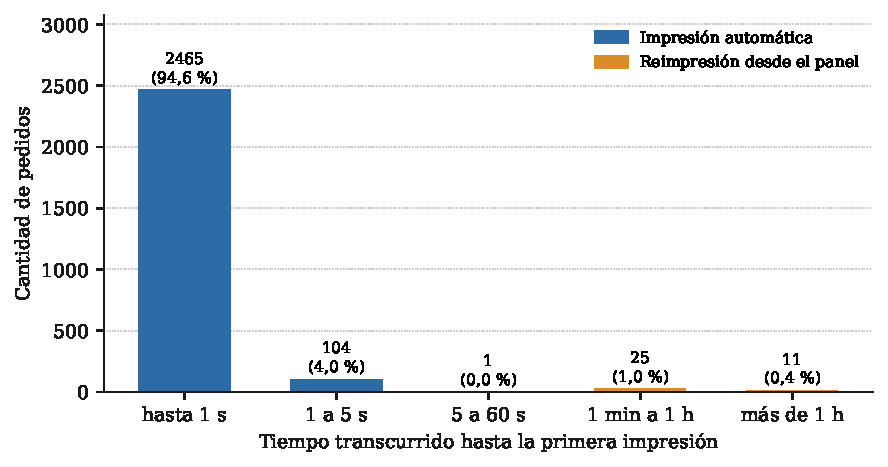
\includegraphics[width=0.9\textwidth]{Figures/latencia_impresion.pdf}
    \caption{Distribución del tiempo transcurrido entre la persistencia del pedido y su primera impresión.}
    \label{fig:latencia_impresion}
\end{figure}

La primera población corresponde a la impresión automática que el sistema dispara al persistir el pedido. La segunda corresponde a la reimpresión diferida que el personal ejecuta desde el panel, en general con precios incluidos, en el momento del despacho. Esa interpretación se confirma al observar que 1321 pedidos registraron exactamente dos impresiones, cantidad superior a los 1113 pedidos con una sola, y que 1621 de las impresiones correctas se emitieron con precios frente a 2717 sin ellos. La doble emisión responde al flujo operativo del comercio, que utiliza un ticket sin precios para el armado del pedido y otro con precios para su entrega.

En la tabla \ref{tab:latencias} se presentan las métricas correspondientes a la población de impresión automática.

\begin{table}[H]
    \centering
    \caption{Latencia de la impresión automática en el borde.}
    \label{tab:latencias}
    \begin{tabular}{L{5.5cm} c}
        \toprule
        \textbf{Métrica} & \textbf{Valor} \\
        \midrule
        Casos analizados & 2569           \\
        Mínimo           & 0,110\,s       \\
        Media            & 0,425\,s       \\
        Mediana          & 0,338\,s       \\
        Percentil 95     & 0,921\,s       \\
        Percentil 99     & 1,475\,s       \\
        Máximo           & 4,220\,s       \\
        \bottomrule
    \end{tabular}
\end{table}

El resultado más significativo no es la mediana sino la dispersión. El peor caso registrado en 50 días de operación fue de 4,22 segundos, y la coincidencia entre media y mediana indica una distribución sin cola apreciable. La actuación física del sistema resultó, por lo tanto, no solo rápida sino predecible.

Ese comportamiento es consecuencia directa del criterio de distribución del cómputo. La orden de impresión recorre un único salto dentro de la red del comercio y no atraviesa Internet, de modo que su latencia queda determinada por la red local y por el tiempo de respuesta de la impresora.

\subsection{Composición de la latencia extremo a extremo}
\label{subsec:composicion_latencia}

La latencia total percibida por el comercio se compone de dos tramos. El primero abarca desde la recepción del mensaje hasta la persistencia del pedido y se resuelve en la nube. El segundo abarca desde la persistencia hasta la emisión del ticket y se resuelve en el borde, con los valores de la sección anterior.

El primer tramo se midió a partir de la duración de las ejecuciones del flujo de interpretación. En la figura \ref{fig:latencia_orquestacion} se presenta su distribución.

\begin{figure}[H]
    \centering
    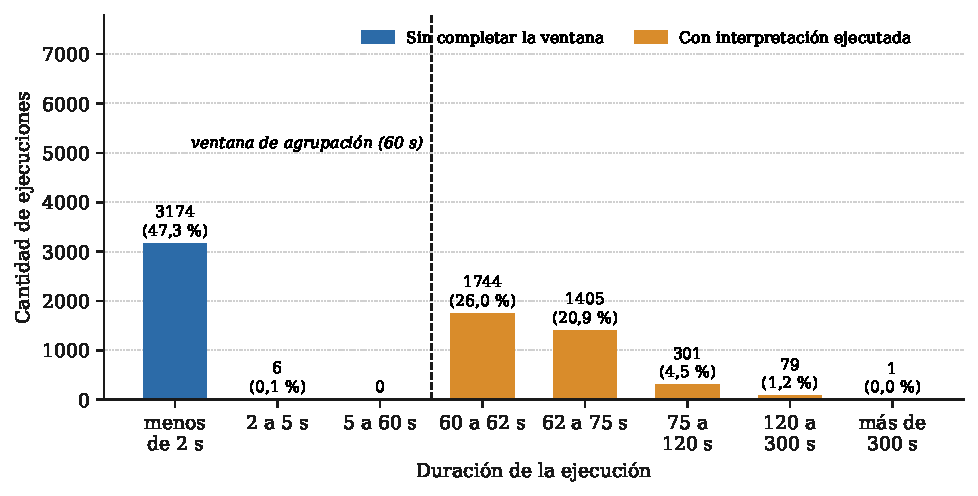
\includegraphics[width=0.9\textwidth]{Figures/latencia_orquestacion.pdf}
    \caption{Distribución de la duración de las ejecuciones del flujo de interpretación de pedidos.}
    \label{fig:latencia_orquestacion}
\end{figure}

La distribución vuelve a presentar dos poblaciones separadas por un intervalo vacío. El 47,39 por ciento de las ejecuciones finalizó en menos de cinco segundos y el 52,61 por ciento restante superó los 60, sin ningún caso registrado entre ambos valores.

La explicación se encuentra en el mecanismo de agrupación de mensajes descripto en la subsección \ref{subsec:criterio_distribucion}. Ese mecanismo no impone una espera fija sino una espera por inactividad. Cada mensaje entrante se incorpora a una lista asociada al cliente y la ejecución aguarda 60 segundos antes de reevaluar el estado de esa lista. Si durante ese lapso llegó un mensaje posterior, la ejecución concluye sin procesar y delega la interpretación en la ejecución más reciente. Si no llegó ninguno, procede a interpretar el conjunto completo y elimina la lista.

La distribución permite entonces distinguir tres comportamientos. Las 3180 ejecuciones que finalizaron en menos de cinco segundos corresponden a mensajes descartados por los filtros previos, que excluyen los mensajes de grupos y los emitidos por el propio comercio. Las 1744 comprendidas entre 60 y 62 segundos corresponden a mensajes sucesivos de un mismo pedido, que concluyeron al detectar la llegada de un mensaje posterior. Las 1786 restantes son las que ejecutaron efectivamente la interpretación, y de ellas 1405 completaron el procesamiento en menos de 15 segundos adicionales a la espera, 301 lo hicieron entre 15 y 60, 79 entre 60 y 240, y una sola superó ese valor.

El tiempo de cómputo de la interpretación se ubica, por lo tanto, en el orden de las unidades de segundo. La demora dominante en el tramo que se resuelve en la nube no proviene del procesamiento sino de la espera deliberada por inactividad del cliente.

El contraste entre ambos tramos constituye el resultado central del trabajo. La etapa que depende de servicios remotos admite una espera de 60 segundos porque su restricción no es de latencia sino de completitud del pedido, mientras que la etapa que ejecuta la actuación física en el borde opera con un máximo de 4,22 segundos y una mediana inferior al medio segundo. La distribución del cómputo asignó a cada entorno la tarea que mejor se ajusta a sus características.

Corresponde precisar qué unidad mide esta distribución, ya que 1786 ejecuciones completaron la interpretación frente a 789 pedidos persistidos, una relación de 2,26 ejecuciones por pedido. La reconstrucción de las agrupaciones que el mecanismo de espera habría formado sobre los 3386 mensajes de la ventana arroja 1801 con un corte de 90 segundos, valor que difiere en menos del uno por ciento de esas 1786 ejecuciones.

La coincidencia establece que cada ejecución de interpretación corresponde a una conversación agrupada y no a un pedido. Las 997 conversaciones restantes son intercambios que superaron los filtros previos pero no derivaron en un encargo, como consultas de precio, confirmaciones y saludos. La duración medida es, en consecuencia, la del procesamiento de una conversación, y el sistema resuelve algo más del doble de conversaciones que de pedidos.

\subsection{Auditoría por formato de entrada}
\label{subsec:ensayo_formatos}

El requerimiento de admitir pedidos en texto, voz, imagen y documento exige comparar el comportamiento del sistema entre esas cuatro modalidades. Ninguna de las dos primeras fuentes de medición lo permite, ya que la base relacional conserva el pedido ya estructurado y no el mensaje que lo originó. La comparación se construyó, en consecuencia, sobre el registro de la plataforma de atención, que sí conserva el tipo de contenido de cada mensaje entrante.

\subsubsection*{Reconstrucción del vínculo entre mensaje y pedido}

Los dos sistemas no comparten identificadores, por lo que la correspondencia entre un mensaje y el pedido se reconstruyó emparejando cada pedido con el último mensaje entrante del mismo contacto anterior a su registro, aprovechando el mecanismo de agrupación por inactividad de la subsección \ref{subsec:composicion_latencia}. La distancia mediana entre ambos es de 72 segundos (primer cuartil 68, tercer cuartil 85), coherente con la espera de 60 segundos más el procesamiento. Se consideraron atribuibles los pedidos con un mensaje precedente a no más de 120 segundos, criterio que alcanza a 3038 de los 3871 pedidos de la ventana (78,48 por ciento).

La cobertura del emparejamiento se mantuvo estable a lo largo del período (mediana diaria del 79 por ciento, mínimo del 61 por ciento), sin días anómalos, lo que descarta que el subconjunto atribuido corresponda a un tramo particular de la operación.

\subsubsection*{Composición del tráfico y resultados por formato}

Durante la ventana de 75 días se recibieron 16\,619 mensajes entrantes de contactos individuales. De ese total, el 77,39 por ciento fue texto, el 12,41 por ciento audio, el 8,29 por ciento imagen, el 1,78 por ciento documento y el 0,14 por ciento video. Las cuatro modalidades previstas por el requerimiento se presentan, por lo tanto, en la operación real y con volumen suficiente para ser comparadas, con la salvedad del video, cuya presencia es marginal.

En la tabla \ref{tab:formatos} se presentan los resultados de la auditoría sobre los 3038 pedidos atribuidos. La categoría mixta reúne los pedidos cuya agrupación combina adjuntos de más de un tipo.

\begin{table}[H]
    \centering
    \caption{Auditoría por formato de entrada sobre los pedidos atribuidos.}
    \label{tab:formatos}
    \begin{tabular}{l c c c c c}
        \toprule
        \textbf{Formato} & \textbf{Pedidos} & \textbf{\%} & \textbf{Ítems} & \textbf{Tasa de asociación} & \textbf{Ítems/pedido} \\
        \midrule
        Texto            & 2013             & 66,26       & 12\,060        & 99,17                       & 5,99                  \\
        Audio            & 563              & 18,53       & 2952           & 99,32                       & 5,24                  \\
        Imagen           & 405              & 13,33       & 4727           & 99,30                       & 11,67                 \\
        Mixto            & 40               & 1,32        & 321            & 98,75                       & 8,03                  \\
        Documento        & 16               & 0,53        & 424            & 98,11                       & 26,50                 \\
        Video            & 1                & 0,03        & 1              & 100,00                      & 1,00                  \\
        \midrule
        Total            & 3038             & 100,00      & 20\,485        & 99,19                       & 6,74                  \\
        \bottomrule
    \end{tabular}
\end{table}

El resultado principal es la ausencia de diferencias apreciables en la tasa de asociación entre las tres modalidades de volumen significativo. El texto alcanza el 99,17 por ciento, el audio el 99,32 y la imagen el 99,30, valores comprendidos en un intervalo de 0,15 puntos porcentuales. El documento presenta el valor más bajo, 98,11 por ciento, pero sobre una base de 16 pedidos que no admite generalización. La interpretación multimodal no introduce, en consecuencia, una penalización medible respecto del texto plano, que constituye el resultado de mayor relevancia para el requerimiento.

El segundo resultado es que el formato sí determina el tamaño del pedido. Un pedido enviado por texto contiene en promedio 5,99 ítems y uno enviado por audio 5,24, mientras que uno enviado por imagen contiene 11,67 y uno enviado como documento 26,50. Las modalidades de imagen y documento concentran los pedidos extensos, que son los que el comercio recibe como lista completa de reposición, y su aporte al volumen total de ítems resulta muy superior al que sugiere su participación en la cantidad de pedidos: la imagen representa el 13,33 por ciento de los pedidos pero el 23,08 por ciento de los ítems.

La combinación de ambos resultados corrige la lectura planteada como hipótesis en la subsección \ref{subsec:items_no_reconocidos}. El error residual no se concentra en la modalidad de imagen. Lo que la imagen concentra son los pedidos extensos con terminología de proveedor, de modo que la asociación entre listas manuscritas y denominaciones no interpretables responde al contenido de esos pedidos y no a una degradación de la interpretación por el hecho de provenir de una fotografía.

\subsubsection*{Limitaciones de la auditoría}

Tres limitaciones acotan el alcance de estos resultados y deben declararse de forma explícita.

La primera es que el indicador es la tasa de asociación con el catálogo, no la exactitud de la interpretación: un ítem asociado puede tener una cantidad o unidad incorrecta que ninguna fuente registra, y verificarlo exigiría contrastar cada pedido contra el mensaje original, viable solo por muestreo manual sobre este volumen.

La segunda es que el tiempo extremo a extremo no puede desagregarse por formato, ya que el registro de ejecuciones no discrimina la modalidad procesada, lo que impide aislar el costo de la transcripción de audio o de la lectura de imagen dentro de la latencia total.

La tercera es que el 21,52 por ciento de los pedidos de la ventana no pudo atribuirse a ningún mensaje próximo. Ese conjunto tiene pedidos más grandes (10,78 ítems) y menor asociación (96,75 por ciento), por lo que su exclusión eleva el valor global de la muestra auditada por encima del 98,45 por ciento real. La comparación entre formatos no se ve afectada porque el sesgo opera por igual sobre todos, pero los valores de la tabla \ref{tab:formatos} no deben leerse como la tasa de asociación del sistema, reportada en la subsección \ref{subsec:items_no_reconocidos}.

\subsection{Ensayo de interfaz}
\label{subsec:ensayo_interfaz}

El acceso al panel sin instalación adicional y su adaptación a distintos tamaños de pantalla se verificaron con un recorrido funcional en Google Chrome, Mozilla Firefox y Microsoft Edge, y en dos anchos de pantalla representativos de un teléfono (375\,px) y una tablet (768\,px).

El recorrido de las vistas de tablero, pedidos, detalle de pedido, productos, clientes y estadísticas no arrojó errores ni advertencias en la consola de ninguno de los tres navegadores. En el ancho de tablet el panel se comportó de forma equivalente al escritorio, dado el tamaño de pantalla similar; el menú lateral se colapsa en un menú desplegable y los controles resultan operables con el dedo. En el ancho de teléfono el panel es utilizable, sin errores ni elementos rotos, aunque algunas vistas con tablas extensas requieren desplazamiento horizontal, una oportunidad de mejora de la experiencia antes que una falla funcional.

El panel cumple, en consecuencia, con el acceso sin instalación adicional y con una adaptación funcional a los tres tamaños de pantalla evaluados. Las capturas del anexo \ref{AppendixA} documentan el estado de las vistas recorridas, de la figura \ref{fig:panel_tablero} a la \ref{fig:panel_metricas}, junto con el ticket emitido en el comercio (figura \ref{fig:ticket_real}).

\subsection{Trazabilidad del pedido}
\label{subsec:trazabilidad}

La trazabilidad se verificó de forma estructural. Cada pedido conserva el conjunto de ítems interpretados, con su denominación original cuando no pudieron asociarse al catálogo, el texto exacto enviado a la impresora y el registro completo de los intentos de impresión con su resultado, su marca temporal y su eventual mensaje de error. El panel permite además acceder desde cada pedido al hilo de la conversación que le dio origen.

La consecuencia práctica de ese diseño es que la totalidad de las mediciones presentadas en este capítulo pudo obtenerse a partir de la propia base de datos del sistema, sin instrumentación adicional. La trazabilidad no solo satisface el requerimiento correspondiente, sino que constituyó el instrumento de medición principal del trabajo.

La cadena presenta, sin embargo, una discontinuidad. El mensaje original recibido del cliente no se persiste en la base relacional, que almacena el pedido ya estructurado, sino que permanece únicamente en la plataforma de atención vinculada al canal de mensajería. La reconstrucción del recorrido completo exige, en consecuencia, consultar dos sistemas distintos.

%----------------------------------------------------------------------------------------
%	SECTION 5
%----------------------------------------------------------------------------------------

\section{Análisis de resultados}
\label{sec:analisis_resultados}

Los ensayos anteriores aportan la evidencia con la que se cierra el capítulo. Esta sección la ordena en tres planos: contrasta cada requerimiento con la medición que lo respalda, reúne las limitaciones que esa medición dejó a la vista y deriva de ellas las mejoras propuestas.

\subsection{Verificación de los requerimientos}
\label{subsec:verificacion_requerimientos}

Los requerimientos se agrupan según la naturaleza de la evidencia. La tabla \ref{tab:verificacion} reúne los que se contrastaron con una medición cuantitativa sobre la operación real.

\begin{table}[H]
    \centering
    \caption{Requerimientos verificados por medición.}
    \label{tab:verificacion}
    \begin{tabular}{c L{5.8cm} L{6.0cm}}
        \toprule
        \textbf{Req.} & \textbf{Evidencia}                                     & \textbf{Resultado}                                                                               \\
        \midrule
        1.2           & Auditoría por formato de entrada.                      & Cuatro formatos en operación; asociación de 99,17 a 99,32 por ciento sin diferencia entre ellos. \\
        1.3           & Tasa de asociación de ítems con el catálogo.           & 98,45 por ciento sobre 29\,457 ítems.                                                            \\
        1.6           & Operaciones de impresión y pedidos sin ticket emitido. & 99,49 por ciento de 4334 operaciones; 15 sin ticket (0,39 por ciento).                           \\
        1.7           & Episodios de pérdida del vínculo con el borde.         & Siete episodios en 50 días, 21 pedidos afectados.                                                \\
        1.11          & Registro de ítems, ticket e impresiones.               & Verificado con una discontinuidad.                                                               \\
        3.1           & Pruebas unitarias automatizadas.                       & No implementadas.                                                                                \\
        3.2           & Tasa de error de la orquestación.                      & 0,10 por ciento sobre 7036 ejecuciones.                                                          \\
        3.3           & Operación en el comercio durante 75 días.              & 3871 pedidos de 202 clientes.                                                                    \\
        3.4           & Impresiones sin fallas atribuibles a la impresora.     & Verificado.                                                                                      \\
        3.5           & Latencia de la actuación en el borde.                  & Mediana de 0,338\,s.                                                                             \\
        \bottomrule
    \end{tabular}
\end{table}

La tabla \ref{tab:verificacion_funcional} reúne los requerimientos verificados por comprobación funcional cuyo resultado aporta algo más que el cumplimiento. Los restantes se omiten por no arrojar un resultado distinto de este: la persistencia y el uso de Redis de las subsecciones \ref{subsec:modelo_datos} y \ref{subsec:agrupacion} (1.4 y 1.5), el panel con sus alertas y su configuración del catálogo de la subsección \ref{subsec:panel} (1.9, 1.10 y 4.2), el acceso sin instalación de la subsección \ref{subsec:ensayo_interfaz} (4.1) y el versionado de los flujos (5.3).

\begin{table}[H]
    \centering
    \caption{Requerimientos verificados de forma funcional.}
    \label{tab:verificacion_funcional}
    \begin{tabular}{c L{5.8cm} L{6.0cm}}
        \toprule
        \textbf{Req.} & \textbf{Evidencia}                                                   & \textbf{Resultado}                                               \\
        \midrule
        1.1           & Recepción y procesamiento continuo de pedidos por WhatsApp.          & Verificado; 3871 pedidos de 202 clientes en 75 días.             \\
        1.8           & Ticket con datos del cliente, productos, aclaraciones, fecha y hora. & Verificado; anexo \ref{AppendixA}, figura \ref{fig:ticket_real}. \\
        4.3           & Adaptación a distintos tamaños de pantalla.                          & Verificado; con \textit{scroll} horizontal en teléfono.          \\
        5.1           & Compatibilidad con la API oficial de WhatsApp Business.              & Diseño compatible; migración no ejecutada.                       \\
        5.2           & Soporte para múltiples dispositivos o cuentas.                       & No evaluado con la evidencia disponible.                         \\
        \bottomrule
    \end{tabular}
\end{table}

El balance es que todos los requerimientos verificables quedaron satisfechos, con una excepción y una salvedad: las pruebas unitarias automatizadas del requerimiento 3.1, cuya función cubrió la operación real sin capacidad de detectar regresiones, y el requerimiento 1.11, verificado con la discontinuidad que introduce la ausencia del mensaje original en la base relacional.

\FloatBarrier

\subsection{Limitaciones detectadas}
\label{subsec:limitaciones}

El conjunto de ensayos permitió identificar seis limitaciones.

La primera es la dependencia del estado del catálogo. La cobertura incompleta y la baja de productos vigentes explican 364 de los 458 ítems no asociados, el 79,48 por ciento: productos incorporados con posterioridad, de almacén y frescos ausentes, dados de baja y las variedades comerciales y códigos de calibre que se retoman en la limitación siguiente. El sistema carece de un mecanismo que anticipe esa condición, de modo que la incorporación ocurre siempre después del primer pedido que la solicita.

La segunda es la cobertura frente a la terminología del comercio mayorista. Las variedades y los códigos de calibre de las listas de proveedor no tienen correspondencia en el catálogo, que registra los productos por su nombre genérico, y concentran 112 casos. Sumados a las 80 denominaciones sin correspondencia interpretable, que dependen de la lectura del mensaje de origen y no de la cobertura, alcanzan el 41,92 por ciento de los ítems no asociados. La distinción importa porque los primeros se resuelven ampliando el catálogo y los segundos, no.

La tercera es la ausencia de reintento automático de la impresión. Los episodios de pérdida de conectividad dejaron 15 pedidos sin ticket, el 0,39 por ciento del total, y su recuperación quedó a cargo del personal, que debió advertir la situación y armar el pedido sin comprobante.

La cuarta es la ausencia de registro del instante de recepción y del formato de origen del mensaje en la base de datos. Esa omisión impide medir la latencia extremo a extremo de forma directa y comparar modalidades de entrada, e introduce la discontinuidad de trazabilidad de la subsección \ref{subsec:trazabilidad}.

La quinta es la ausencia de identificación del operador en el registro de impresiones. El campo previsto permaneció sin valor en todos los casos, por lo que la distinción entre impresión automática y reimpresión manual debió inferirse de la distribución de latencias.

La sexta es la ausencia de pruebas automatizadas, señalada en la subsección \ref{subsec:estrategia_verificacion}, que impide detectar regresiones de manera anticipada.

\subsection{Mejoras propuestas}
\label{subsec:mejoras_ensayos}

De las limitaciones anteriores se desprenden seis mejoras concretas, que se retoman en el capítulo \ref{Chapter5}.

La primera es una vista de ítems no asociados en el panel, ordenada por frecuencia, que permita dar de alta los productos faltantes de forma sistemática y no reactiva. La medición indica que 123 de los 458 casos, el 0,42 por ciento de los ítems procesados, se habrían evitado con el alta oportuna de productos que luego se incorporaron o estaban dados de baja. Corresponde además revisar el criterio de baja, ya que los clientes siguen pidiendo artículos desactivados.

La segunda es sumar al catálogo las variedades comerciales y los códigos de calibre de los proveedores, vinculados a su producto genérico, lo que permitiría interpretar las listas de proveedor con la precisión que ya alcanzan los pedidos minoristas.

La tercera es una cola de impresiones pendientes con reintento automático al restablecerse el vínculo. Los episodios registrados muestran que la indisponibilidad del enlace se resuelve sola en plazos acotados, de modo que un reintento diferido habría emitido los 15 tickets faltantes sin intervención del personal. Es la mejora de mayor impacto sobre la confiabilidad percibida.

La cuarta es agregar a la tabla de pedidos el instante de recepción, el formato de origen y una referencia al mensaje original, lo que permitiría medir la latencia extremo a extremo y el desempeño por formato de forma permanente, y cerraría la discontinuidad de trazabilidad.

La quinta es el registro efectivo del operador que dispara cada impresión desde el panel, lo que separaría de forma explícita las dos poblaciones que este capítulo debió distinguir por inferencia.

La sexta es la revisión del intervalo de espera por inactividad. El tiempo de interpretación se ubica en el orden de las unidades de segundo, muy por debajo de los 60 segundos de cada ciclo de espera, y 1744 de las 3530 ejecuciones que ingresaron al mecanismo concluyeron sin procesar por la llegada de un mensaje posterior. Reducir el intervalo bajaría la latencia percibida en los pedidos de un único mensaje sin afectar la agrupación de los fragmentados; medir antes la distribución del tiempo entre mensajes sucesivos de un mismo cliente permitiría fijar ese valor con fundamento empírico.
% !TEX root = ../memorianueva.tex
% Chapter Template

\chapter{Conclusiones} % Main chapter title

\label{Chapter5} % Change X to a consecutive number; for referencing this chapter elsewhere, use \ref{ChapterX}

En el presente capítulo se valora el trabajo realizado a la luz de los objetivos planteados y de la evidencia reunida en el capítulo \ref{Chapter4}. Se analiza el grado de cumplimiento de los requerimientos, la fidelidad de la ejecución respecto de la planificación original, el comportamiento de los riesgos identificados y la utilidad de las técnicas empleadas. El capítulo cierra con las líneas de trabajo que se desprenden de los resultados obtenidos.

%----------------------------------------------------------------------------------------
%	SECTION 1
%----------------------------------------------------------------------------------------

\section{Conclusiones generales}

El trabajo produjo un sistema que se encuentra en operación continua en el comercio para el que fue concebido. Esa circunstancia constituye el principal aporte, ya que los resultados presentados no provienen de un banco de pruebas sino del uso sostenido por parte de sus destinatarios durante 75 días, con 3871 pedidos de 202 clientes y 29457 ítems interpretados.

\subsection{Grado de cumplimiento de los objetivos}

Los objetivos específicos formulados en la sección \ref{sec:objetivos} se alcanzaron en su totalidad. Los logros concretos son los siguientes:

\begin{itemize}
	\item Se automatizó la captura de pedidos en las cuatro modalidades que el canal admite. La auditoría de la sección \ref{subsec:ensayo_formatos} verificó que texto, audio e imagen se interpretan con tasas de asociación comprendidas entre el 99,17 y el 99,32 por ciento, sin penalización medible de las modalidades multimodales respecto del texto plano.
	\item Se alcanzó una tasa de asociación de ítems con el catálogo del 98,45 por ciento sobre 29457 ítems, y el análisis de los 458 casos restantes demostró que el 79,48 por ciento de ellos responde a limitaciones de cobertura del catálogo y no a errores de interpretación.
	\item Se implementó la trazabilidad completa del pedido, que resultó suficiente para obtener la totalidad de las mediciones de este trabajo sin instrumentación adicional.
	\item Se automatizó la impresión en el borde con una latencia de mediana 0,338 segundos y máximo 4,22 segundos, sobre 4334 operaciones con una tasa de éxito del 99,49 por ciento.
	\item Se estableció la comunicación segura entre la nube y el nodo de borde mediante un túnel, cuyo comportamiento se caracterizó en 7 episodios de indisponibilidad a lo largo de 50 días.
	\item Se construyó el panel web, que se incorporó a la operación diaria y que además habilitó el mecanismo de realimentación del catálogo descripto más adelante.
	\item Se validó el sistema en condiciones reales, criterio de aceptación que operó de manera efectiva mediante el uso sostenido por parte del comercio.
\end{itemize}

De los requerimientos verificados en la sección \ref{subsec:verificacion_requerimientos}, uno solo no se satisfizo: el que preveía la implementación de pruebas unitarias automatizadas. La verificación se resolvió en su reemplazo mediante la operación real, estrategia que aportó una cobertura de casos superior pero que no detecta regresiones de manera anticipada ni permite aislar la causa de una falla. La incorporación de esas pruebas queda como la deuda técnica más relevante del trabajo. Un segundo requerimiento, el de trazabilidad, se verificó con una salvedad: el mensaje original no se persiste en la base relacional, de modo que la reconstrucción del recorrido completo exige consultar dos sistemas distintos.

\subsection{Fidelidad respecto de la planificación}

La ejecución se apartó de la planificación en el ordenamiento de las etapas antes que en su contenido. El historial del repositorio de desarrollo sitúa el inicio de la construcción el 20 de abril de 2026 y su última intervención el 1 de septiembre del mismo año. La actividad no se distribuyó de manera uniforme: se concentró en una primera etapa intensiva durante la segunda quincena de abril, en la que quedó definida la arquitectura, y en un segundo bloque durante junio, que absorbió la mayor parte del desarrollo del panel web. Los meses posteriores registran intervenciones puntuales de ajuste sobre la interfaz de programación y sobre los flujos de orquestación. Corresponde advertir que la frecuencia de las confirmaciones del repositorio documenta la cronología de la construcción, pero no constituye una medida del esfuerzo dedicado, de modo que no permite contrastar el total contra las 600 horas previstas en la planificación.

La desviación de mayor consecuencia fue deliberada y consistió en adelantar la puesta en producción respecto del final del desarrollo. El sistema entró en operación el 1 de junio de 2026 y registró su primer pedido el 4 de junio, cuando el panel web todavía se encontraba en construcción y el comercio aún no contaba con la impresora térmica. Durante las cuatro primeras semanas la capa de captura e interpretación operó con el volumen completo de pedidos mientras los resultados se volcaban a un archivo de texto que el personal consultaba de forma manual. La automatización de la impresión se habilitó recién el 29 de junio, una vez verificada la calidad de la interpretación.

El efecto de esa decisión fue favorable en dos sentidos. Redujo el riesgo de la puesta en marcha, ya que ningún fallo de interpretación pudo traducirse en un ticket erróneo durante el período de observación, y aportó cuatro semanas de datos reales que orientaron la ampliación del catálogo antes de que el sistema operara de forma autónoma. Su costo fue una mayor carga operativa para el personal durante ese lapso.

\subsection{Comportamiento de los riesgos identificados}

De los cinco riesgos previstos en la planificación, dos se manifestaron durante el período de operación.

El riesgo de fallas de integración entre la plataforma de orquestación, la interfaz de programación y los servicios de inteligencia artificial no se materializó. Sobre 7036 ejecuciones se registraron 7 fallas, equivalentes al 0,10 por ciento, y cada una de esas ejecuciones involucra a la totalidad de los componentes de la cadena.

El riesgo de caídas del servidor local de impresión sí se manifestó, y constituye el caso en que el plan de mitigación resultó inefectivo por no haberse implementado. Se registraron 7 episodios de pérdida del vínculo en 50 días, que afectaron a 21 pedidos y dejaron 15 sin ticket emitido, equivalentes al 0,39 por ciento de los procesados. La mitigación prevista consistía en un mecanismo de supervisión y reinicio automático del proceso en el nodo de borde, que no llegó a incorporarse. La resolución quedó en consecuencia a cargo del personal, que debió advertir la falta del comprobante y armar el pedido consultando el panel. Corresponde señalar que la evidencia recogida sugiere una mitigación más adecuada que la prevista: dado que la indisponibilidad se resuelve por sí sola en plazos acotados, una cola de reintentos en la nube habría emitido los 15 tickets faltantes sin intervención alguna, y lo habría hecho con independencia de la causa de la caída.

El riesgo de baja calidad de los mensajes recibidos se manifestó de forma parcial y con un alcance menor al previsto. Los 458 ítems que el sistema no pudo asociar representan el 1,55 por ciento del total, y de ellos solo 80 corresponden a denominaciones sin correspondencia interpretable. La auditoría por formato demostró además que ese error residual no depende de la modalidad del mensaje, de modo que la interpretación multimodal resultó más robusta de lo que la planificación anticipaba. La mitigación efectiva no fue ninguna de las previstas, sino un mecanismo emergente que se describe en el apartado siguiente.

El riesgo de pérdida de datos en la base no se manifestó. No se detectaron inconsistencias durante el período y el relevamiento de la infraestructura no registra reinicios acumulados en ninguno de los contenedores en servicio.

El riesgo de sobrecostos en el consumo de los servicios de inteligencia artificial tampoco se manifestó. Su evaluación exigió recurrir a los paneles de facturación de los dos proveedores, dado que el gasto no queda registrado en ninguna de las fuentes internas del sistema. Sobre la ventana comprendida entre el 4 de junio y el 17 de agosto de 2026 el consumo conjunto totalizó 236,29 dólares estadounidenses, equivalentes a 3,15 dólares diarios y a un costo unitario de 6,1 centavos de dólar por pedido. La planificación no fijó un valor de corte para este rubro, de modo que el contraste no puede establecerse contra un presupuesto previo, pero la magnitud observada resulta holgadamente compatible con la restricción de bajo costo que orienta el trabajo y respalda la decisión de consumir los modelos como servicio en lugar de ejecutarlos sobre infraestructura propia, sobre todo si se considera que ese gasto incluye la redundancia de dos modelos sobre cada imagen y su posterior reconciliación.

Como observación transversal, el dimensionamiento de la infraestructura resultó holgado. El servidor virtual, con cuatro núcleos y 16 gigabytes de memoria, sostuvo la totalidad de los servicios con una carga media inferior a la centésima parte de su capacidad de cómputo, un consumo de memoria de 3,6 gigabytes y una ocupación de disco del 11 por ciento, tras 227 días de servicio ininterrumpido. La base relacional del sistema ocupa alrededor de 12 megabytes luego de 4934 pedidos y 37931 ítems, mientras que el registro de ejecuciones de la plataforma de orquestación supera los dos gigabytes y medio. Esa desproporción, de más de dos órdenes de magnitud, explica por sí sola la necesidad de la purga automática que restringió la ventana de análisis de la orquestación a catorce días.

\subsection{Técnicas empleadas}

Tres técnicas resultaron decisivas para el desarrollo.

La primera fue la construcción de un servidor de impresión simulado, que reproduce la interfaz del servidor real y registra el ticket en lugar de imprimirlo. Permitió desarrollar y depurar la totalidad de la cadena sin disponer del hardware, que se adquirió cuando el resto del sistema ya se encontraba en operación.

La segunda fue el despliegue escalonado descripto más arriba, que separó la puesta en producción de la interpretación de la puesta en producción de la actuación física.

La tercera fue el lazo de realimentación del catálogo. El panel destaca los ítems que no pudieron asociarse, y el personal del comercio los empleó para ampliar el catálogo de forma progresiva. El caso del huevo resulta ilustrativo: acumuló 55 ocurrencias no asociadas entre el 10 de junio y el 12 de julio, fecha en que el producto se dio de alta, y a partir de entonces no volvió a registrar ningún fallo. Esa técnica no estaba prevista en la planificación y emergió del uso, pero constituyó la mitigación efectiva del riesgo de calidad de la interpretación.

En sentido inverso, dos decisiones no rindieron lo esperado. La ausencia de pruebas automatizadas obligó a diferir toda verificación hasta la operación real, lo que resultó viable en este proyecto por su escala pero no constituye una práctica extrapolable. Y la redundancia de dos modelos de proveedores distintos sobre cada imagen, con un tercer modelo que reconcilia sus lecturas, agrega costo y latencia sin que el trabajo haya podido medir su aporte, dado que el sistema no conserva las lecturas individuales previas a la reconciliación.

%----------------------------------------------------------------------------------------
%	SECTION 2
%----------------------------------------------------------------------------------------
\section{Próximos pasos}

Las líneas de continuación se ordenan según su impacto sobre la operación.

La primera es la implementación de una cola de impresiones pendientes con reintento automático al restablecerse el vínculo con el nodo de borde. Es la mejora de mayor impacto sobre la confiabilidad percibida, ya que habría evitado la totalidad de los 15 pedidos que quedaron sin comprobante, y su alcance es superior al del mecanismo de supervisión previsto en la planificación por resolver el problema con independencia de su causa.

La segunda es la extensión del modelo de datos para incorporar el instante de recepción del mensaje, su formato de origen y una referencia al mensaje original. Esa modificación cerraría la discontinuidad de la cadena de trazabilidad y convertiría en permanentes dos mediciones que este trabajo debió reconstruir por inferencia: la latencia extremo a extremo y el desempeño desagregado por formato de entrada.

La tercera es la ampliación del catálogo con las variedades comerciales y los códigos de calibre de los proveedores, junto con una vista del panel que ordene por frecuencia los ítems no asociados. Ambas medidas atacan el 79,48 por ciento del error residual que responde a limitaciones de cobertura, y transformarían en sistemático el lazo de realimentación que hoy opera de manera reactiva.

La cuarta es la revisión del intervalo de espera por inactividad. La medición demostró que el tiempo de interpretación se ubica en el orden de las unidades de segundo, muy por debajo de los sesenta que dura cada ciclo de espera, de modo que su reducción disminuiría la latencia percibida en los pedidos enviados en un único mensaje. Una caracterización previa de la distribución del tiempo entre mensajes sucesivos de un mismo cliente permitiría fijar ese valor con fundamento empírico.

La quinta es la incorporación de pruebas automatizadas sobre los módulos de interpretación e impresión, junto con el registro del operador que dispara cada impresión desde el panel. La primera cancela la deuda técnica señalada; la segunda separaría de forma explícita las dos poblaciones de impresiones que este trabajo debió distinguir por inferencia.

Por último, la evidencia reunida sugiere una línea de trabajo que excede el alcance original. El sistema resuelve algo más del doble de conversaciones que de pedidos, ya que interpreta consultas, confirmaciones y saludos que no derivan en un encargo. Ese volumen, hoy descartado, constituye información sobre la demanda y sobre la interacción con los clientes que el sistema podría aprovechar.


%----------------------------------------------------------------------------------------
% Apéndices
%----------------------------------------------------------------------------------------

\appendix

% Incluir apéndices desde archivos separados si es necesario
%% !TEX root = ../memorianueva.tex
% Appendix A

% Este anexo es solo de figuras: sin estos ajustes LaTeX exige un mínimo de
% texto por página y deja una sola imagen por hoja, con mucho espacio en blanco.
\renewcommand{\topfraction}{0.95}
\renewcommand{\bottomfraction}{0.95}
\renewcommand{\textfraction}{0.05}
\renewcommand{\floatpagefraction}{0.85}
\setcounter{topnumber}{4}
\setcounter{bottomnumber}{4}
\setcounter{totalnumber}{6}

\chapter{Capturas del sistema en operación}
\label{AppendixA}

En este anexo se incluyen las imágenes reales del sistema en funcionamiento: el ticket generado y las vistas del panel web de control.

\section{Ticket impreso}

\begin{figure}[htbp]
    \centering
    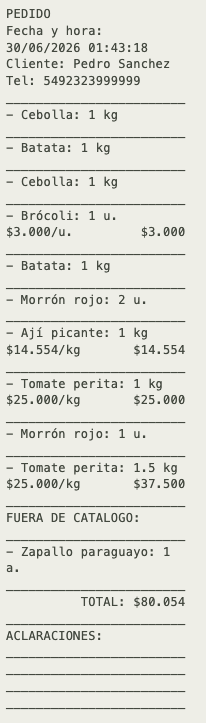
\includegraphics[height=0.52\textheight]{Figures/ticket_impreso.png}
    \caption{Ticket real generado por el sistema e impreso en el comercio.}
    \label{fig:ticket_real}
\end{figure}

\FloatBarrier

\section{Panel web de control}

\begin{figure}[htbp]
    \centering
    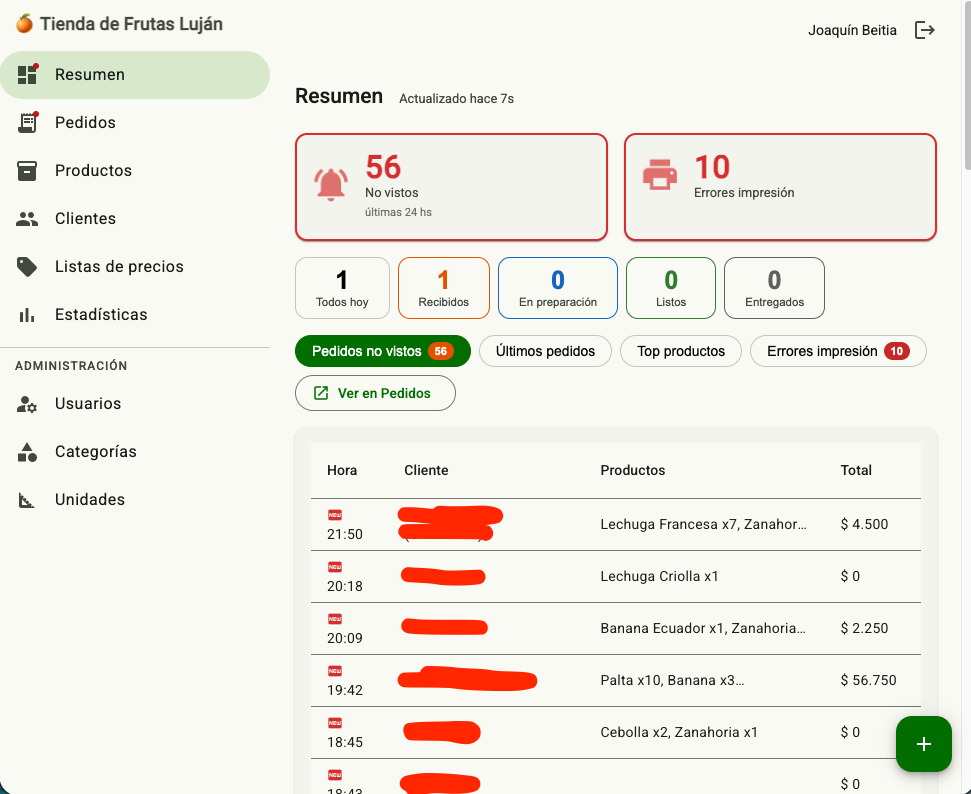
\includegraphics[width=0.82\textwidth]{Figures/panel_dashboard.png}
    \caption{Tablero principal del panel de control.}
    \label{fig:panel_tablero}
\end{figure}

\begin{figure}[htbp]
    \centering
    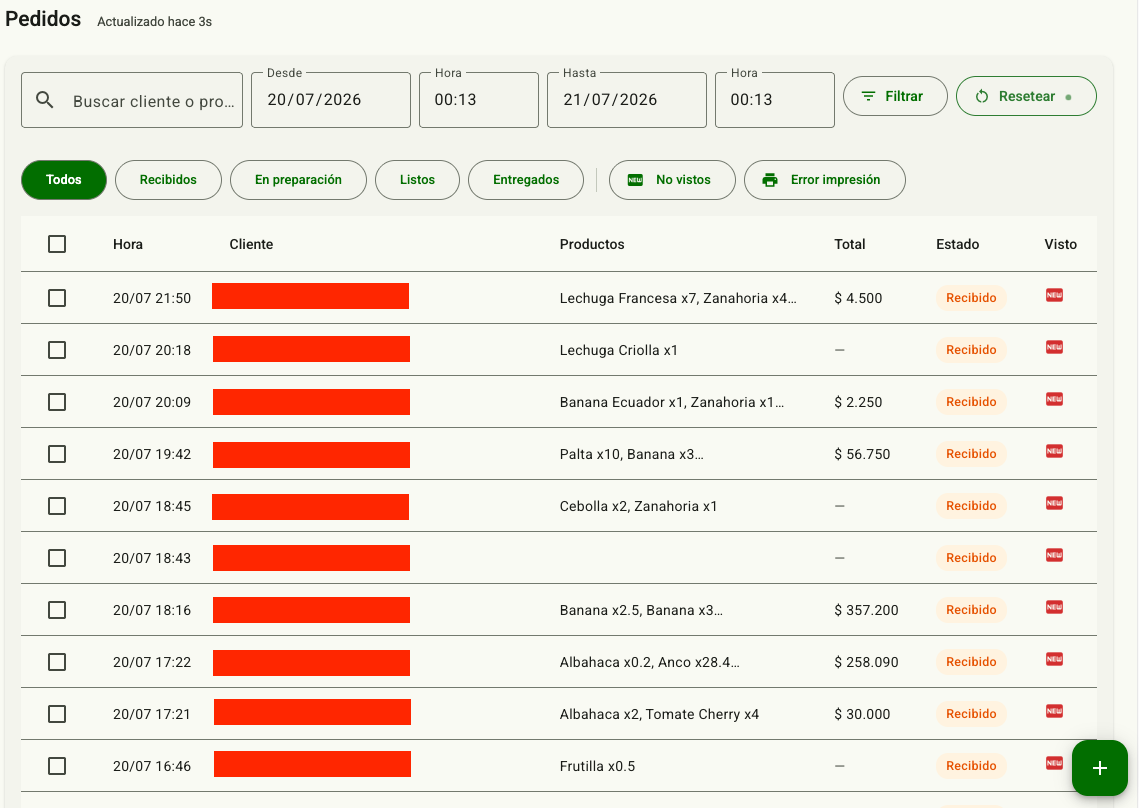
\includegraphics[width=0.82\textwidth]{Figures/panel_pedidos.png}
    \caption{Listado de pedidos con sus filtros de búsqueda.}
    \label{fig:panel_pedidos}
\end{figure}

\begin{figure}[htbp]
    \centering
    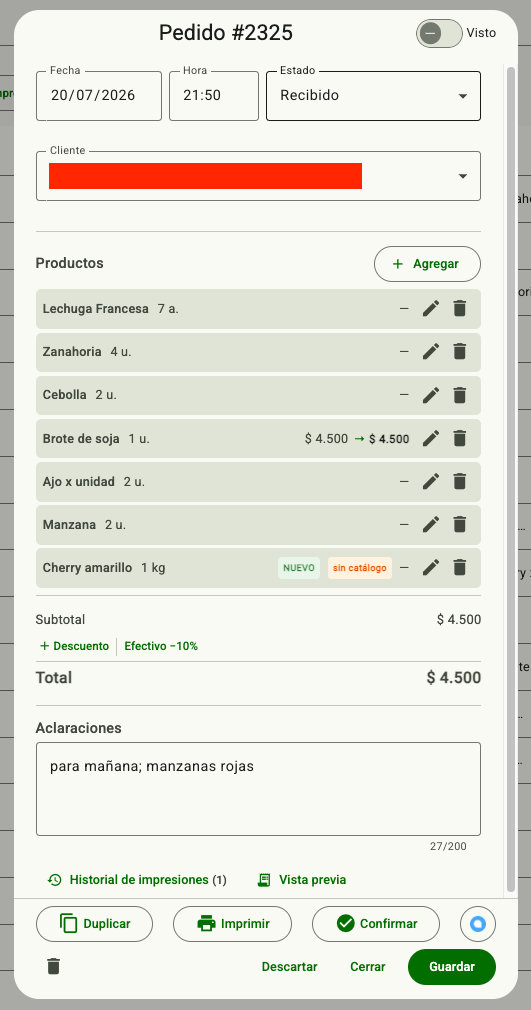
\includegraphics[width=0.4\textwidth]{Figures/panel_detalle_pedido.png}
    \caption{Detalle de un pedido, con edición de ítems y acceso al mensaje original.}
    \label{fig:panel_detalle}
\end{figure}

\begin{figure}[htbp]
    \centering
    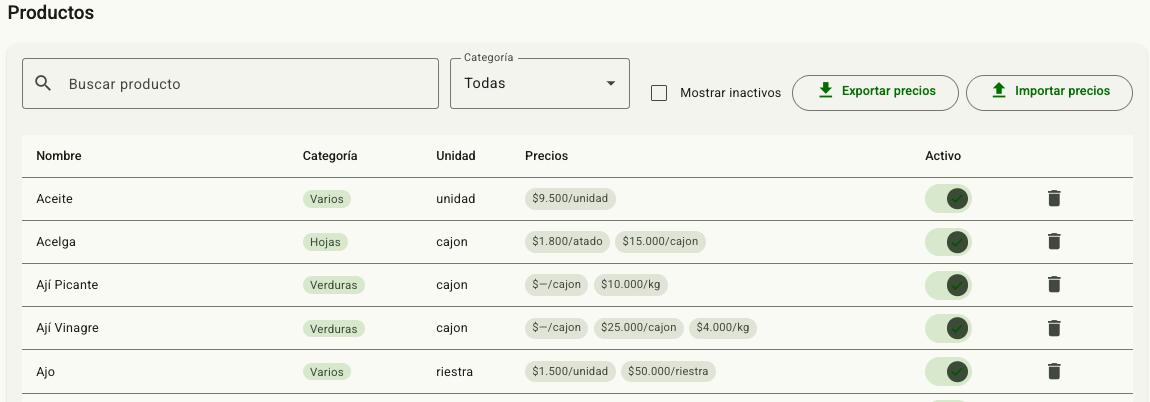
\includegraphics[width=\textwidth]{Figures/panel_productos.png}
    \caption{Administración del catálogo de productos.}
    \label{fig:panel_catalogo}
\end{figure}

\begin{figure}[htbp]
    \centering
    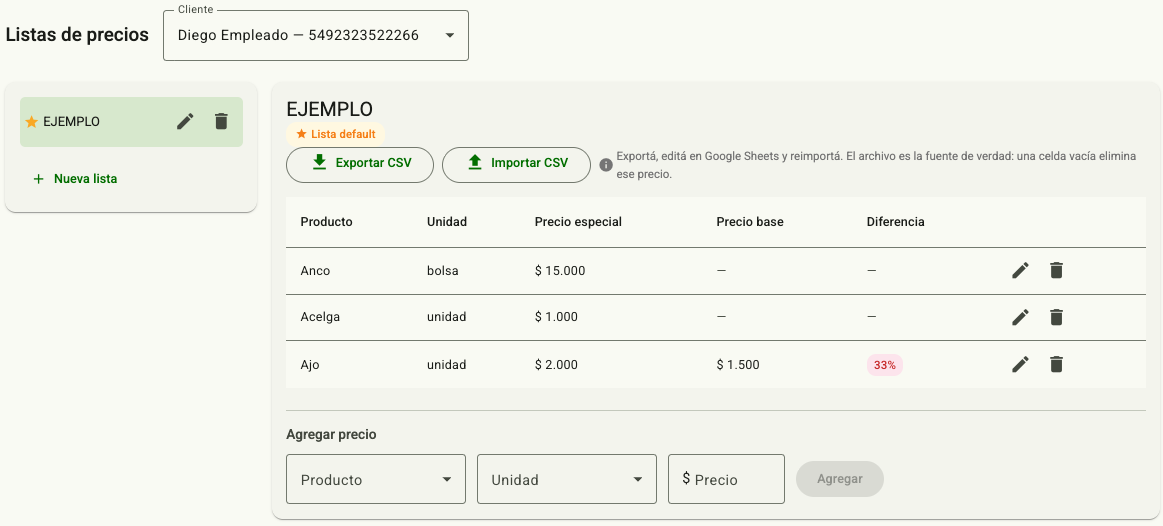
\includegraphics[width=\textwidth]{Figures/panel_listas_precios.png}
    \caption{Administración de las listas de precios de un cliente.}
    \label{fig:panel_precios}
\end{figure}

\begin{figure}[htbp]
    \centering
    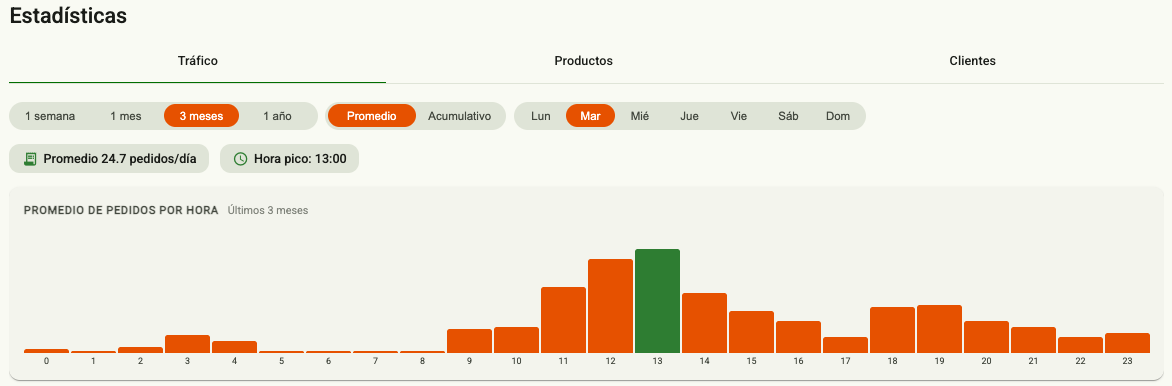
\includegraphics[width=\textwidth]{Figures/panel_estadisticas.png}
    \caption{Vista de métricas de operación del comercio.}
    \label{fig:panel_metricas}
\end{figure}

\FloatBarrier


%----------------------------------------------------------------------------------------
% Bibliografía
%----------------------------------------------------------------------------------------

\renewcommand{\bibname}{Bibliografía} % Para asegurarte de que el título sea correcto
\phantomsection % Necesario para que el enlace del marcador sea correcto

\printbibliography[heading=bibintoc]

\end{document}






